\author{Chaya2766}
\title{humanity of the third millenium \linebreak under assumption of exponential growth}
\date{last updated \today}

\documentclass[a4paper]{article}
\usepackage[margin=3cm]{geometry}
\usepackage{graphicx}
\usepackage{pgfplots}

\usepackage{hyperref}
\hypersetup{
	colorlinks=true,
	linkcolor=blue,
	filecolor=magenta,
	urlcolor=cyan,
	hyperindex=true,
	linktocpage=true,%makes the page number be the link in the index
}
\usepackage{listings}
\lstset{
	basicstyle=\tiny\ttfamily,
	columns=fullflexible,
	keepspaces=true,
	breaklines=true,
	frame=single,
	showstringspaces=true,
	tabsize=4,
	showspaces=true,
	showtabs=true,
}

\renewcommand{\arraystretch}{1.2}



\begin{document}
	\sffamily
	\hyphenchar\font=-1
	\sloppy
	
	\maketitle
	
	\textbf{
		\sloppy
		\hyphenchar\font=-1
	}
	
	\vfill
	
	\begin{abstract}
		An exponential curve had been matched to the relevant data between the years 1900 and 2021/2023 in these areas: total population, life expectancy, GDP (global total \& per capita), energy consumption (global total \& per capita).
		
		\medskip
		
		Results are presented as plots showing the curve and the real data together, as well as plots \& tables showing resulting values for the future between years 2000 and 3000.
		
		\medskip
		
		This is in no way an argument for or against the idea that humanity in the real world will follow a general trend of exponential growth into the future, but rather merely a computation of the values that would result from applying that assumption for use in worldbuilding.
	\end{abstract}
	
	\vfill
	
	\begin{quote}
		\begin{center}
			\textbf{DISCLAIMER AND WARNING}
		\end{center}
		
		This is not a scientific paper or engineering advice.
		This document is only intended as creative world‑building and has not been peer‑reviewed or approved for any practical application.
		Use of these ideas in real‑world designs or other serious application is entirely at the reader’s discretion and risk.
	\end{quote}
	
	%\noindent \rule{\linewidth}{1pt}
	\vfill
	
	\tableofcontents
	
	\pagebreak

	
	\section{exponential human population growth}
	
	Below in red I've plotted the population across past years since 1900, well past the industrial revolution, my data comes from Our World In Data. In blue ploted is a function:
	
	\begin{center}
		{\large $ y = 1627883132 \times 1.01314982563501^{x-1900} $}
	\end{center}
	
	Which is simply exponential growth from the starting number of people (1627883132) in 1900 that both plots begin at, multiplied by 1.01314982563501 for every passing year to represent $\approx 1.315\%$ increase in population per year.
	
	\bigskip
	
	%\begin{center}
		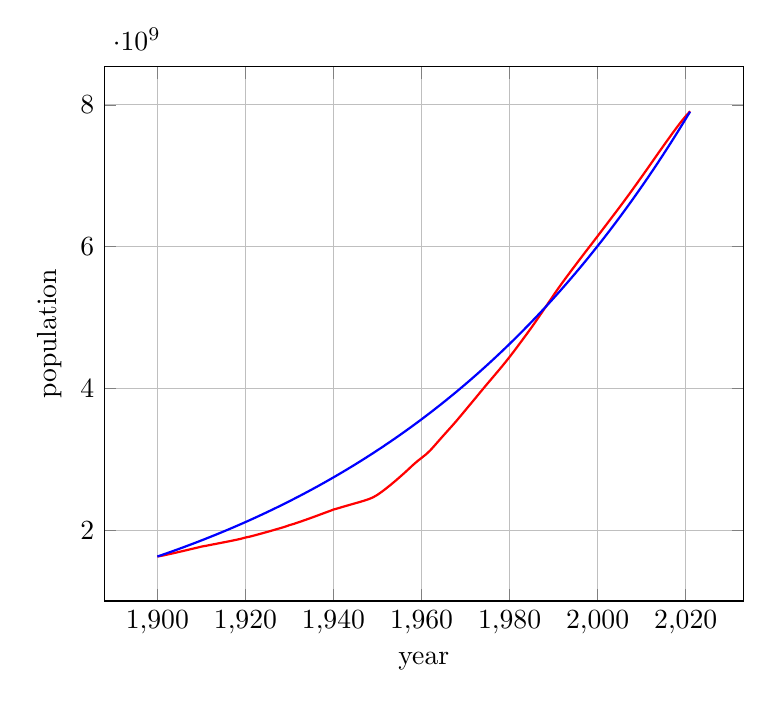
\begin{tikzpicture}
			\begin{axis}[
				width=0.8\linewidth,
				xlabel=year,
				ylabel=population,
				%ymode=log,
				%xmin=1, xmax=100,
				%ymin=0, ymax=10,
				grid=both,
				minor grid style={gray!25},
				major grid style={gray!50},
				]
				\addplot[red, thick] coordinates {
					(1900, 1627883132)
					(1901, 1638647517)
					(1902, 1651840077)
					(1903, 1665703540)
					(1904, 1679752718)
					(1905, 1693984163)
					(1906, 1708411294)
					(1907, 1723032738)
					(1908, 1737874788)
					(1909, 1752122665)
					(1910, 1767847653)
					(1911, 1778784032)
					(1912, 1791197929)
					(1913, 1803056235)
					(1914, 1815104863)
					(1915, 1827290389)
					(1916, 1839559287)
					(1917, 1851899055)
					(1918, 1864869126)
					(1919, 1878650358)
					(1920, 1895682150)
					(1921, 1908748639)
					(1922, 1924826120)
					(1923, 1941636900)
					(1924, 1958716901)
					(1925, 1976068839)
					(1926, 1993719848)
					(1927, 2011689749)
					(1928, 2029682397)
					(1929, 2048513689)
					(1930, 2070596353)
					(1931, 2088429965)
					(1932, 2109357892)
					(1933, 2131029147)
					(1934, 2152969392)
					(1935, 2175184808)
					(1936, 2197830032)
					(1937, 2220878589)
					(1938, 2244005191)
					(1939, 2266483407)
					(1940, 2290871362)
					(1941, 2307736768)
					(1942, 2326734579)
					(1943, 2344581440)
					(1944, 2362439908)
					(1945, 2380167769)
					(1946, 2397811266)
					(1947, 2416694412)
					(1948, 2437259361)
					(1949, 2463242071)
					(1950, 2499322112)
					(1951, 2543130368)
					(1952, 2590270976)
					(1953, 2640278784)
					(1954, 2691979264)
					(1955, 2746072064)
					(1956, 2801002752)
					(1957, 2857866752)
					(1958, 2916108032)
					(1959, 2970292224)
					(1960, 3019233536)
					(1961, 3068370688)
					(1962, 3126686720)
					(1963, 3195779328)
					(1964, 3267212288)
					(1965, 3337112064)
					(1966, 3406416896)
					(1967, 3475448064)
					(1968, 3546810880)
					(1969, 3620655360)
					(1970, 3695390208)
					(1971, 3770163200)
					(1972, 3844800768)
					(1973, 3920251392)
					(1974, 3995516928)
					(1975, 4069437184)
					(1976, 4142505728)
					(1977, 4215772416)
					(1978, 4289657600)
					(1979, 4365582848)
					(1980, 4444007936)
					(1981, 4524627456)
					(1982, 4607984640)
					(1983, 4691884032)
					(1984, 4775836160)
					(1985, 4861730816)
					(1986, 4950063104)
					(1987, 5040984576)
					(1988, 5132294144)
					(1989, 5223704064)
					(1990, 5316175872)
					(1991, 5406245888)
					(1992, 5492686336)
					(1993, 5577433600)
					(1994, 5660727808)
					(1995, 5743219712)
					(1996, 5825145344)
					(1997, 5906481152)
					(1998, 5987312640)
					(1999, 6067758592)
					(2000, 6148898816)
					(2001, 6230747136)
					(2002, 6312407552)
					(2003, 6393898496)
					(2004, 6475751424)
					(2005, 6558176256)
					(2006, 6641416192)
					(2007, 6725948416)
					(2008, 6811597312)
					(2009, 6898306048)
					(2010, 6985603072)
					(2011, 7073125376)
					(2012, 7161697792)
					(2013, 7250593280)
					(2014, 7339013632)
					(2015, 7426597376)
					(2016, 7513474048)
					(2017, 7599822336)
					(2018, 7683789824)
					(2019, 7764951040)
					(2020, 7840952832)
					(2021, 7909295104)
				};
				\addplot[blue, thick, domain=1900:2021, samples=100]  {1627883132*pow(1.01314982563501,x-1900)};
			\end{axis}
		\end{tikzpicture}
	%\end{center}

	\pagebreak
	
	Let us consider the following millenium, and go all the way out to the year 3000 using this same roughly $1.315\%$ growth per year:
	
	%\begin{center}
		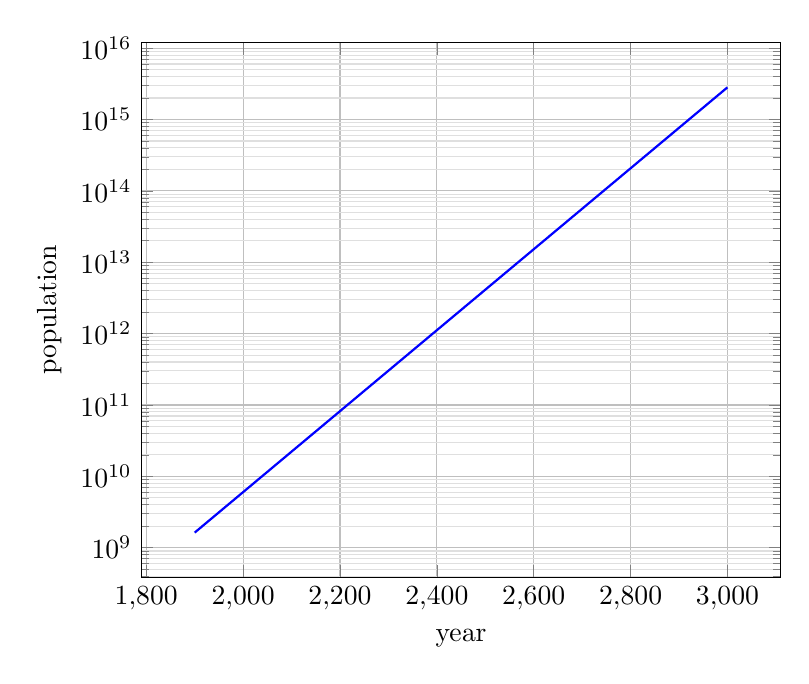
\begin{tikzpicture}
			\begin{axis}[
				width=0.8\linewidth,
				xlabel=year,
				ylabel=population,
				ymode=log,
				%xmin=1, xmax=100,
				%ymin=0, ymax=10,
				grid=both,
				minor grid style={gray!25},
				major grid style={gray!50},
				]
				
				\addplot[blue, thick, domain=1900:3000, samples=100]  {1627883132*pow(1.01314982563501,x-1900)};
			\end{axis}
		\end{tikzpicture}
		
		\bigskip
		
		Here are some precise numbers to be extracted from this:
		
	\begin{center}		
		\begin{tabular}{c | c | c | c }
			year & exact population & rough population & order of magnitude \\\hline
			2000 & 6 011 607 607 & $6\times10^9$ & billions \\\hline
			2050 & 11 552 456 090 & $11.5\times10^9$ & tens of billions \\\hline
			2100 & 22 200 258 306 & $22.2\times10^9$ & tens of billions \\\hline
			2150 & 42 662 050 824 & $42.7\times10^9$ & tens of billions \\\hline
			2200 & 81 983 306 474 & $82\times10^9$ & tens of billions \\\hline
			2250 & 157 546 634 788 & $157.5\times10^9$ & hundreds of billions \\\hline
			2300 & 302 756 051 205 & $302.8\times10^9$ & hundreds of billions \\\hline
			2350 & 581 803 772 987 & $581.8\times10^9$ & hundreds of billions \\\hline
			2400 & 1 118 047 447 489 & $1.12\times10^{12}$ & trillions \\\hline
			2450 & 2 148 542 434 542 & $2.15\times10^{12}$ & trillions \\\hline
			2500 & 4 128 836 037 678 & $4.13\times10^{12}$ & trillions \\\hline
			2600 & 15 247 373 503 074 & $15.2\times10^{12}$ & tens of trillions \\\hline
			2700 & 56 307 006 773 998 & $56.3\times10^{12}$ & tens of trillions \\\hline
			2800 & 207 936 075 758 080 & $207.9\times10^{12}$ & hundreds of trillions \\\hline
			2900 & 767 886 877 297 784 & $767.9\times10^{12}$ & hundreds of trillions \\\hline
			3000 & 2 835 728 500 580 920 & $2.8\times10^{15}$ & quadrillions \\
		\end{tabular}
	\end{center}
	
	\pagebreak
	
	\small
	
	\noindent
	\begin{tabular}{|c|c|}
		\hline
		year & population \\
		\hline
		2025 & 8.3336E+09 \\
		\hline
		2030 & 8.8961E+09 \\
		\hline
		2035 & 9.4966E+09 \\
		\hline
		2040 & 1.0138E+10 \\
		\hline
		2045 & 1.0822E+10 \\
		\hline
		2050 & 1.1552E+10 \\
		\hline
		2055 & 1.2332E+10 \\
		\hline
		2060 & 1.3165E+10 \\
		\hline
		2065 & 1.4053E+10 \\
		\hline
		2070 & 1.5002E+10 \\
		\hline
		2075 & 1.6015E+10 \\
		\hline
		2080 & 1.7096E+10 \\
		\hline
		2085 & 1.8250E+10 \\
		\hline
		2090 & 1.9481E+10 \\
		\hline
		2095 & 2.0796E+10 \\
		\hline
		2100 & 2.2200E+10 \\
		\hline
		2105 & 2.3699E+10 \\
		\hline
		2110 & 2.5298E+10 \\
		\hline
		2115 & 2.7006E+10 \\
		\hline
		2120 & 2.8829E+10 \\
		\hline
		2125 & 3.0775E+10 \\
		\hline
		2130 & 3.2852E+10 \\
		\hline
		2135 & 3.5070E+10 \\
		\hline
		2140 & 3.7437E+10 \\
		\hline
		2145 & 3.9964E+10 \\
		\hline
		2150 & 4.2662E+10 \\
		\hline
		2155 & 4.5542E+10 \\
		\hline
		2160 & 4.8616E+10 \\
		\hline
		2165 & 5.1898E+10 \\
		\hline
		2170 & 5.5401E+10 \\
		\hline
		2175 & 5.9140E+10 \\
		\hline
		2180 & 6.3132E+10 \\
		\hline
		2185 & 6.7394E+10 \\
		\hline
		2190 & 7.1943E+10 \\
		\hline
		2195 & 7.6799E+10 \\
		\hline
		2200 & 8.1983E+10 \\
		\hline
		2205 & 8.7517E+10 \\
		\hline
		2210 & 9.3425E+10 \\
		\hline
		2215 & 9.9731E+10 \\
		\hline
		2220 & 1.0646E+11 \\
		\hline
		2225 & 1.1365E+11 \\
		\hline
		2230 & 1.2132E+11 \\
		\hline
		2235 & 1.2951E+11 \\
		\hline
		2240 & 1.3825E+11 \\
		\hline
		2245 & 1.4758E+11 \\
		\hline
		2250 & 1.5755E+11 \\
		\hline
		2255 & 1.6818E+11 \\
		\hline
		2260 & 1.7953E+11 \\
		\hline
		2265 & 1.9165E+11 \\
		\hline
	\end{tabular}
	\hfill
	\begin{tabular}{|c|c|}
		\hline
		year & population \\
		\hline
		2270 & 2.0459E+11 \\
		\hline
		2275 & 2.1840E+11 \\
		\hline
		2280 & 2.3314E+11 \\
		\hline
		2285 & 2.4888E+11 \\
		\hline
		2290 & 2.6568E+11 \\
		\hline
		2295 & 2.8361E+11 \\
		\hline
		2300 & 3.0276E+11 \\
		\hline
		2305 & 3.2319E+11 \\
		\hline
		2310 & 3.4501E+11 \\
		\hline
		2315 & 3.6830E+11 \\
		\hline
		2320 & 3.9316E+11 \\
		\hline
		2325 & 4.1970E+11 \\
		\hline
		2330 & 4.4803E+11 \\
		\hline
		2335 & 4.7827E+11 \\
		\hline
		2340 & 5.1055E+11 \\
		\hline
		2345 & 5.4501E+11 \\
		\hline
		2350 & 5.8180E+11 \\
		\hline
		2355 & 6.2108E+11 \\
		\hline
		2360 & 6.6300E+11 \\
		\hline
		2365 & 7.0775E+11 \\
		\hline
		2370 & 7.5553E+11 \\
		\hline
		2375 & 8.0653E+11 \\
		\hline
		2380 & 8.6097E+11 \\
		\hline
		2385 & 9.1908E+11 \\
		\hline
		2390 & 9.8112E+11 \\
		\hline
		2395 & 1.0474E+12 \\
		\hline
		2400 & 1.1180E+12 \\
		\hline
		2405 & 1.1935E+12 \\
		\hline
		2410 & 1.2741E+12 \\
		\hline
		2415 & 1.3601E+12 \\
		\hline
		2420 & 1.4519E+12 \\
		\hline
		2425 & 1.5499E+12 \\
		\hline
		2430 & 1.6545E+12 \\
		\hline
		2435 & 1.7662E+12 \\
		\hline
		2440 & 1.8854E+12 \\
		\hline
		2445 & 2.0127E+12 \\
		\hline
		2450 & 2.1485E+12 \\
		\hline
		2455 & 2.2936E+12 \\
		\hline
		2460 & 2.4484E+12 \\
		\hline
		2465 & 2.6137E+12 \\
		\hline
		2470 & 2.7901E+12 \\
		\hline
		2475 & 2.9784E+12 \\
		\hline
		2480 & 3.1795E+12 \\
		\hline
		2485 & 3.3941E+12 \\
		\hline
		2490 & 3.6232E+12 \\
		\hline
		2495 & 3.8678E+12 \\
		\hline
		2500 & 4.1288E+12 \\
		\hline
		2505 & 4.4075E+12 \\
		\hline
		2510 & 4.7051E+12 \\
		\hline
	\end{tabular}
	\hfill
	\begin{tabular}{|c|c|}
		\hline
		year & population \\
		\hline
		2515 & 5.0226E+12 \\
		\hline
		2520 & 5.3617E+12 \\
		\hline
		2525 & 5.7236E+12 \\
		\hline
		2530 & 6.1100E+12 \\
		\hline
		2535 & 6.5224E+12 \\
		\hline
		2540 & 6.9627E+12 \\
		\hline
		2545 & 7.4326E+12 \\
		\hline
		2550 & 7.9343E+12 \\
		\hline
		2555 & 8.4699E+12 \\
		\hline
		2560 & 9.0417E+12 \\
		\hline
		2565 & 9.6520E+12 \\
		\hline
		2570 & 1.0304E+13 \\
		\hline
		2575 & 1.0999E+13 \\
		\hline
		2580 & 1.1741E+13 \\
		\hline
		2585 & 1.2534E+13 \\
		\hline
		2590 & 1.3380E+13 \\
		\hline
		2595 & 1.4283E+13 \\
		\hline
		2600 & 1.5247E+13 \\
		\hline
		2605 & 1.6277E+13 \\
		\hline
		2610 & 1.7375E+13 \\
		\hline
		2615 & 1.8548E+13 \\
		\hline
		2620 & 1.9800E+13 \\
		\hline
		2625 & 2.1137E+13 \\
		\hline
		2630 & 2.2563E+13 \\
		\hline
		2635 & 2.4086E+13 \\
		\hline
		2640 & 2.5712E+13 \\
		\hline
		2645 & 2.7448E+13 \\
		\hline
		2650 & 2.9301E+13 \\
		\hline
		2655 & 3.1279E+13 \\
		\hline
		2660 & 3.3390E+13 \\
		\hline
		2665 & 3.5644E+13 \\
		\hline
		2670 & 3.8050E+13 \\
		\hline
		2675 & 4.0618E+13 \\
		\hline
		2680 & 4.3360E+13 \\
		\hline
		2685 & 4.6287E+13 \\
		\hline
		2690 & 4.9411E+13 \\
		\hline
		2695 & 5.2747E+13 \\
		\hline
		2700 & 5.6307E+13 \\
		\hline
		2705 & 6.0108E+13 \\
		\hline
		2710 & 6.4165E+13 \\
		\hline
		2715 & 6.8496E+13 \\
		\hline
		2720 & 7.3120E+13 \\
		\hline
		2725 & 7.8056E+13 \\
		\hline
		2730 & 8.3324E+13 \\
		\hline
		2735 & 8.8949E+13 \\
		\hline
		2740 & 9.4953E+13 \\
		\hline
		2745 & 1.0136E+14 \\
		\hline
		2750 & 1.0820E+14 \\
		\hline
		2755 & 1.1551E+14 \\
		\hline
	\end{tabular}
	\hfill
	\begin{tabular}{|c|c|}
		\hline
		year & population \\
		\hline
		2760 & 1.2331E+14 \\
		\hline
		2765 & 1.3163E+14 \\
		\hline
		2770 & 1.4051E+14 \\
		\hline
		2775 & 1.5000E+14 \\
		\hline
		2780 & 1.6012E+14 \\
		\hline
		2785 & 1.7093E+14 \\
		\hline
		2790 & 1.8247E+14 \\
		\hline
		2795 & 1.9479E+14 \\
		\hline
		2800 & 2.0794E+14 \\
		\hline
		2805 & 2.2197E+14 \\
		\hline
		2810 & 2.3696E+14 \\
		\hline
		2815 & 2.5295E+14 \\
		\hline
		2820 & 2.7002E+14 \\
		\hline
		2825 & 2.8825E+14 \\
		\hline
		2830 & 3.0771E+14 \\
		\hline
		2835 & 3.2848E+14 \\
		\hline
		2840 & 3.5065E+14 \\
		\hline
		2845 & 3.7432E+14 \\
		\hline
		2850 & 3.9959E+14 \\
		\hline
		2855 & 4.2656E+14 \\
		\hline
		2860 & 4.5536E+14 \\
		\hline
		2865 & 4.8609E+14 \\
		\hline
		2870 & 5.1890E+14 \\
		\hline
		2875 & 5.5393E+14 \\
		\hline
		2880 & 5.9132E+14 \\
		\hline
		2885 & 6.3124E+14 \\
		\hline
		2890 & 6.7385E+14 \\
		\hline
		2895 & 7.1933E+14 \\
		\hline
		2900 & 7.6789E+14 \\
		\hline
		2905 & 8.1972E+14 \\
		\hline
		2910 & 8.7505E+14 \\
		\hline
		2915 & 9.3412E+14 \\
		\hline
		2920 & 9.9717E+14 \\
		\hline
		2925 & 1.0645E+15 \\
		\hline
		2930 & 1.1363E+15 \\
		\hline
		2935 & 1.2130E+15 \\
		\hline
		2940 & 1.2949E+15 \\
		\hline
		2945 & 1.3823E+15 \\
		\hline
		2950 & 1.4756E+15 \\
		\hline
		2955 & 1.5752E+15 \\
		\hline
		2960 & 1.6816E+15 \\
		\hline
		2965 & 1.7951E+15 \\
		\hline
		2970 & 1.9163E+15 \\
		\hline
		2975 & 2.0456E+15 \\
		\hline
		2980 & 2.1837E+15 \\
		\hline
		2985 & 2.3311E+15 \\
		\hline
		2990 & 2.4884E+15 \\
		\hline
		2995 & 2.6564E+15 \\
		\hline
		3000 & 2.8357E+15 \\
		\hline
	\end{tabular}
	
	\normalsize
	
	\pagebreak
	
	\section{exponential life expectancy at birth}
	
	Below in red I've ploted the global average life expectancy at birth between years 1900 and 2021 according to Our World In Data, and in blue an exponential function:
	
	\begin{center}
		{\large $ y = 32 \times 1.006613662^{x-1900} $}
	\end{center}
	
	Which represents a starting point at year 1900 with 32 years life expectancy at birth, and growth of roughly 0.66\% per year.
	
	\medskip
	
	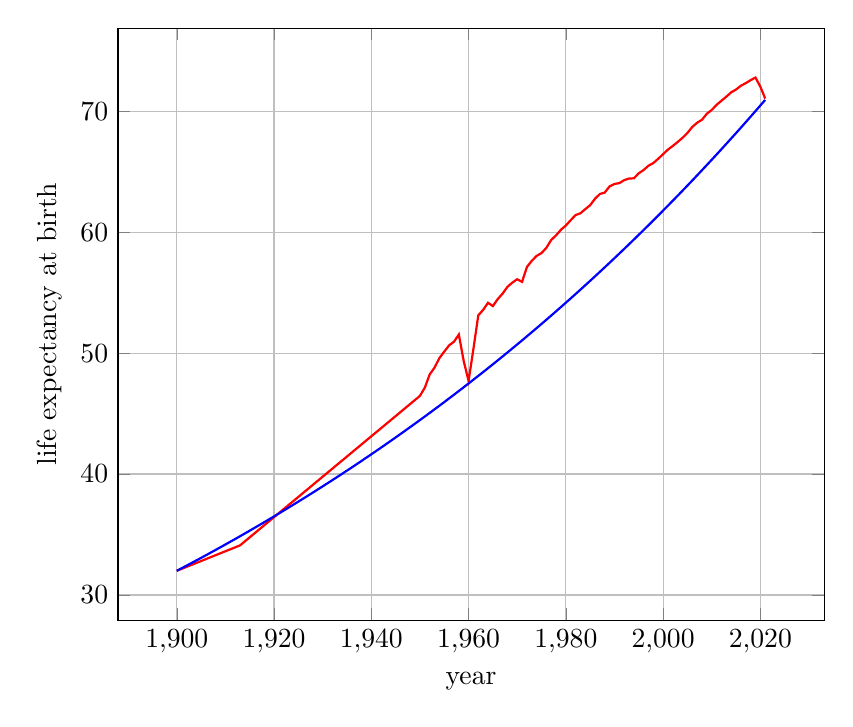
\begin{tikzpicture}
		\begin{axis}[
			width=0.87\linewidth,
			xlabel=year,
			ylabel=life expectancy at birth,
			%ymode=log,
			%xmin=1, xmax=100,
			%ymin=0, ymax=10,
			grid=both,
			minor grid style={gray!25},
			major grid style={gray!50},
			]
			\addplot[red, thick] coordinates {
				(1900,32)
				(1913,34.1)
				(1950,46.4643)
				(1951,47.144)
				(1952,48.2311)
				(1953,48.8024)
				(1954,49.5919)
				(1955,50.1229)
				(1956,50.6425)
				(1957,50.9448)
				(1958,51.537)
				(1959,49.3453)
				(1960,47.6972)
				(1961,50.3587)
				(1962,53.1245)
				(1963,53.5761)
				(1964,54.1638)
				(1965,53.8924)
				(1966,54.472)
				(1967,54.9203)
				(1968,55.486)
				(1969,55.8286)
				(1970,56.112)
				(1971,55.8924)
				(1972,57.1231)
				(1973,57.6327)
				(1974,58.0422)
				(1975,58.2754)
				(1976,58.7107)
				(1977,59.3652)
				(1978,59.7402)
				(1979,60.2037)
				(1980,60.5524)
				(1981,60.9915)
				(1982,61.4165)
				(1983,61.5651)
				(1984,61.907)
				(1985,62.2356)
				(1986,62.7665)
				(1987,63.1585)
				(1988,63.2806)
				(1989,63.7919)
				(1990,63.9879)
				(1991,64.0583)
				(1992,64.3027)
				(1993,64.4369)
				(1994,64.4588)
				(1995,64.8766)
				(1996,65.1429)
				(1997,65.5007)
				(1998,65.7215)
				(1999,66.0735)
				(2000,66.4525)
				(2001,66.8336)
				(2002,67.1373)
				(2003,67.46)
				(2004,67.8074)
				(2005,68.2047)
				(2006,68.7027)
				(2007,69.0508)
				(2008,69.3014)
				(2009,69.7965)
				(2010,70.1088)
				(2011,70.5303)
				(2012,70.8725)
				(2013,71.2072)
				(2014,71.5649)
				(2015,71.8004)
				(2016,72.1102)
				(2017,72.3267)
				(2018,72.5759)
				(2019,72.7897)
				(2020,72.0361)
				(2021,71.0479)
			};
			\addplot[blue, thick, domain=1900:2021, samples=100]  {32*pow(1.006613662,x-1900)};
		\end{axis}
	\end{tikzpicture}
	
	\medskip
	
	I should say, at least to my eye, the real data very much does not feel like it follows exponential growth, rather it looks more like it follows simple linear growth, but even more than that I would say the shape of the curve here is just very hard to guess because it doesn't even remotely look like any of the simple mathematical functions I know.
	
	\bigskip
	
	\noindent
	\begin{minipage}{0.5\linewidth}
		In the years before 1900 which I had not included above for industrial revolution reasons it becomes pretty much flat, showing little change as the years pass, making the actual curve look more like 2 straight lines that touch each other at an angle rather than any kind of gradual, let alone exponential growth.
	\end{minipage}\hfill
	\begin{minipage}{0.45\linewidth}
		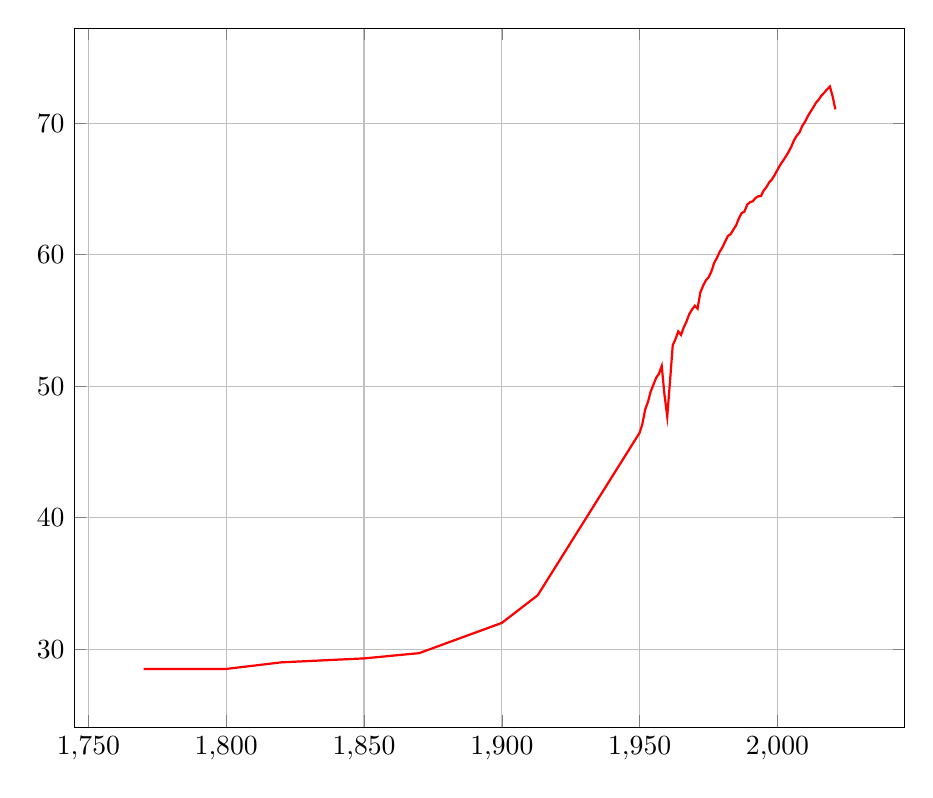
\begin{tikzpicture}
			\begin{axis}[
				width=\linewidth,
				%xlabel=year,
				%ylabel=life expectancy at birth,
				%ymode=log,
				%xmin=1, xmax=100,
				%ymin=0, ymax=10,
				grid=both,
				minor grid style={gray!25},
				major grid style={gray!50},
				]
				\addplot[red, thick] coordinates {
					(1770,28.5)
					(1800,28.5)
					(1820,29)
					(1850,29.3)
					(1870,29.7)
					(1900,32)
					(1913,34.1)
					(1950,46.4643)
					(1951,47.144)
					(1952,48.2311)
					(1953,48.8024)
					(1954,49.5919)
					(1955,50.1229)
					(1956,50.6425)
					(1957,50.9448)
					(1958,51.537)
					(1959,49.3453)
					(1960,47.6972)
					(1961,50.3587)
					(1962,53.1245)
					(1963,53.5761)
					(1964,54.1638)
					(1965,53.8924)
					(1966,54.472)
					(1967,54.9203)
					(1968,55.486)
					(1969,55.8286)
					(1970,56.112)
					(1971,55.8924)
					(1972,57.1231)
					(1973,57.6327)
					(1974,58.0422)
					(1975,58.2754)
					(1976,58.7107)
					(1977,59.3652)
					(1978,59.7402)
					(1979,60.2037)
					(1980,60.5524)
					(1981,60.9915)
					(1982,61.4165)
					(1983,61.5651)
					(1984,61.907)
					(1985,62.2356)
					(1986,62.7665)
					(1987,63.1585)
					(1988,63.2806)
					(1989,63.7919)
					(1990,63.9879)
					(1991,64.0583)
					(1992,64.3027)
					(1993,64.4369)
					(1994,64.4588)
					(1995,64.8766)
					(1996,65.1429)
					(1997,65.5007)
					(1998,65.7215)
					(1999,66.0735)
					(2000,66.4525)
					(2001,66.8336)
					(2002,67.1373)
					(2003,67.46)
					(2004,67.8074)
					(2005,68.2047)
					(2006,68.7027)
					(2007,69.0508)
					(2008,69.3014)
					(2009,69.7965)
					(2010,70.1088)
					(2011,70.5303)
					(2012,70.8725)
					(2013,71.2072)
					(2014,71.5649)
					(2015,71.8004)
					(2016,72.1102)
					(2017,72.3267)
					(2018,72.5759)
					(2019,72.7897)
					(2020,72.0361)
					(2021,71.0479)
				};
			\end{axis}
		\end{tikzpicture}
	\end{minipage}
	
	
	\pagebreak
	
	Once again, let's extend this into the future, but for reasons you will see below I'm only going to extend this out to the year 2200 this time, and since the range is small enough for the real data to be visible I am including it again in red.
	
	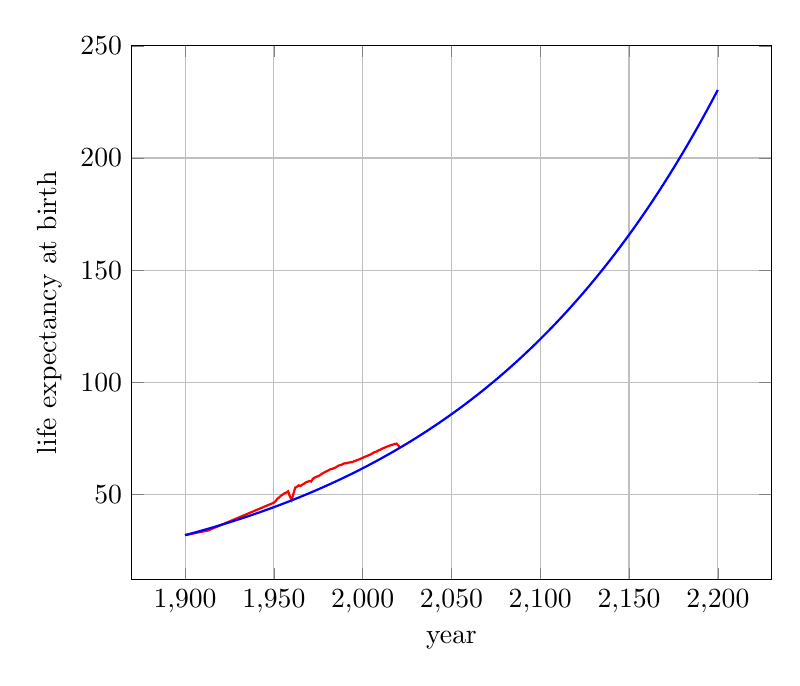
\begin{tikzpicture}
		\begin{axis}[
			width=0.8\linewidth,
			xlabel=year,
			ylabel=life expectancy at birth,
			%ymode=log,
			%xmin=1, xmax=100,
			%ymin=0, ymax=10,
			grid=both,
			minor grid style={gray!25},
			major grid style={gray!50},
			]
			\addplot[red, thick] coordinates {
				(1900,32)
				(1913,34.1)
				(1950,46.4643)
				(1951,47.144)
				(1952,48.2311)
				(1953,48.8024)
				(1954,49.5919)
				(1955,50.1229)
				(1956,50.6425)
				(1957,50.9448)
				(1958,51.537)
				(1959,49.3453)
				(1960,47.6972)
				(1961,50.3587)
				(1962,53.1245)
				(1963,53.5761)
				(1964,54.1638)
				(1965,53.8924)
				(1966,54.472)
				(1967,54.9203)
				(1968,55.486)
				(1969,55.8286)
				(1970,56.112)
				(1971,55.8924)
				(1972,57.1231)
				(1973,57.6327)
				(1974,58.0422)
				(1975,58.2754)
				(1976,58.7107)
				(1977,59.3652)
				(1978,59.7402)
				(1979,60.2037)
				(1980,60.5524)
				(1981,60.9915)
				(1982,61.4165)
				(1983,61.5651)
				(1984,61.907)
				(1985,62.2356)
				(1986,62.7665)
				(1987,63.1585)
				(1988,63.2806)
				(1989,63.7919)
				(1990,63.9879)
				(1991,64.0583)
				(1992,64.3027)
				(1993,64.4369)
				(1994,64.4588)
				(1995,64.8766)
				(1996,65.1429)
				(1997,65.5007)
				(1998,65.7215)
				(1999,66.0735)
				(2000,66.4525)
				(2001,66.8336)
				(2002,67.1373)
				(2003,67.46)
				(2004,67.8074)
				(2005,68.2047)
				(2006,68.7027)
				(2007,69.0508)
				(2008,69.3014)
				(2009,69.7965)
				(2010,70.1088)
				(2011,70.5303)
				(2012,70.8725)
				(2013,71.2072)
				(2014,71.5649)
				(2015,71.8004)
				(2016,72.1102)
				(2017,72.3267)
				(2018,72.5759)
				(2019,72.7897)
				(2020,72.0361)
				(2021,71.0479)
			};
			\addplot[blue, thick, domain=1900:2200, samples=100]  {32*pow(1.006613662,x-1900)};
		\end{axis}
	\end{tikzpicture}
	
	Here are some precise numbers to be extracted from this:
	
	%	\begin{center}
		%		\begin{tabular}{Sc | Sc | Sc }
			%			year & life expectancy at birth & increase over previous year \\\hline
			%			2000 & 61.86 y & 0.4065 y \\\hline
			%			2025 & 72.95 y & 0.4793 y \\\hline
			%			2050 & 86 y & 0.5651 y \\\hline
			%			2075 & 101.42 y & 0.6664 y \\\hline
			%			2100 & 119.59 y & 0.7858 y \\\hline
			%			2137 & 152.63 y & 1 y \\
			%		\end{tabular}
		%	\end{center}
	
	\begin{center}
		\begin{tabular}{c | c | c }
			year & life expectancy at birth & increase over previous year \\\hline
			2020 & 70.58 y & 0.4637 y \\\hline
			2030 & 75.39 y & 0.4953 y \\\hline
			2040 & 80.53 y & 0.5291 y \\\hline
			2050 & 86 y & 0.5651 y \\\hline
			2060 & 91.88 y & 0.6036 y \\\hline
			2070 & 98.14 y & 0.6448 y \\\hline
			2080 & 104.82 y & 0.6887 y \\\hline
			2090 & 111.97 y & 0.7356 y \\\hline
			2100 & 119.59 y & 0.7858 y \\\hline
			2110 & 127.74 y & 0.8393 y \\\hline
			2120 & 136.45 y & 0.8965 y \\\hline
			2130 & 145.75 y & 0.9576 y \\\hline
			2137 & 152.63 y & 1 y \\
		\end{tabular}
	\end{center}
	
	It is a little pointless to continue past the year 2137 in this model as at this year, life expectancy begins to grow by more than 1 year every year, granting everyone born past that point theoretical immortality. The more widely known name for this effect is "longevity escape velocity" for those more interested.
	
	\pagebreak
	
	\section{exponential GDP per capita growth}
	
	Going into this chapter it's important to remember that GDP per capita is not the same as the amount of money an average person earns, nor even really implies that money still exists in whatever society we are contemplating here - you might think of it as factoring in not just your personal earnings but costs to maintain the roads you drive on or the bus you take to work \& such.
	
	\medskip
	
	Below in red I've ploted the global average GDP per capita (expressed in international dollars at 2017 prices) between years 1900 and 2022 according to Our World In Data, and in blue an exponential function:
	
	\begin{center}
		{\large $ y = 2700 \times 1.015450028^{x-1900} $}
	\end{center}
	
	Which represents a starting point at year 1900 with 2700 international-\$, and growth of roughly 1.545\% per year.
	
	\medskip
	
	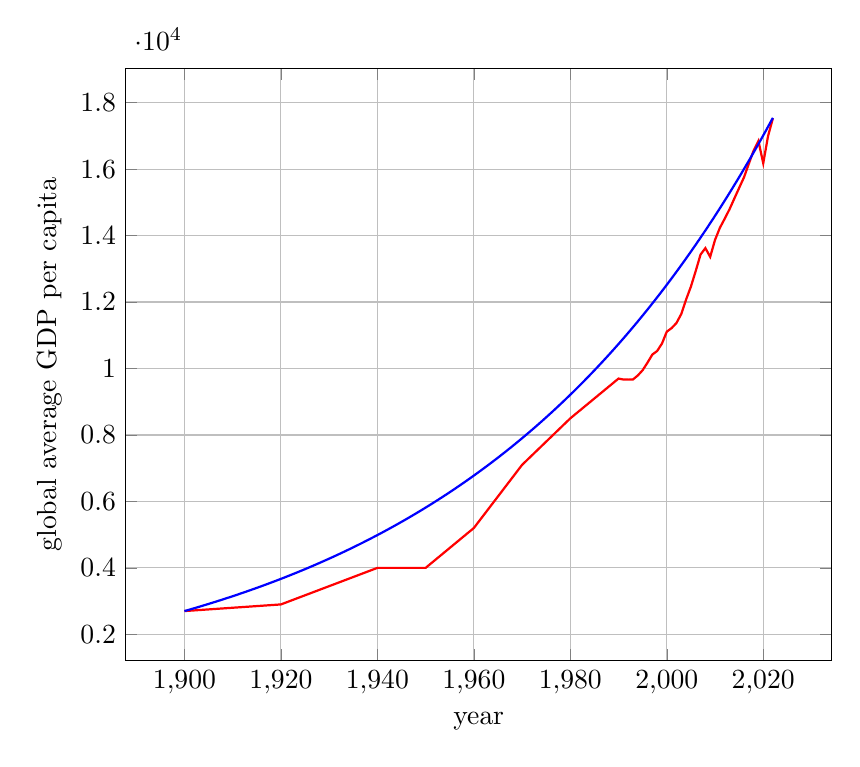
\begin{tikzpicture}
		\begin{axis}[
			width=0.87\linewidth,
			xlabel=year,
			ylabel=global average GDP per capita,
			%ymode=log,
			%xmin=1, xmax=100,
			%ymin=0, ymax=10,
			grid=both,
			minor grid style={gray!25},
			major grid style={gray!50},
			]
			\addplot[red, thick] coordinates {
				(1900,2700)
				(1920,2900)
				(1940,4000)
				(1950,4000)
				(1960,5200)
				(1970,7100)
				(1980,8500)
				(1990,9697.508)
				(1991,9667.7)
				(1992,9665.21)
				(1993,9670.078)
				(1994,9791.423)
				(1995,9949.668)
				(1996,10175.511)
				(1997,10418.802)
				(1998,10526.854)
				(1999,10749.006)
				(2000,11108.324)
				(2001,11215.04)
				(2002,11367.639)
				(2003,11637.828)
				(2004,12074.206)
				(2005,12463.141)
				(2006,12933.736)
				(2007,13428.616)
				(2008,13622.655)
				(2009,13359.558)
				(2010,13868.406)
				(2011,14230.719)
				(2012,14504.989)
				(2013,14789.622)
				(2014,15112.653)
				(2015,15433.18)
				(2016,15750.084)
				(2017,16156.354)
				(2018,16558.998)
				(2019,16847.46)
				(2020,16175.776)
				(2021,16997.135)
				(2022,17527)
			};
			\addplot[blue, thick, domain=1900:2022, samples=100]  {2700*pow(1.015450028,x-1900)};
		\end{axis}
	\end{tikzpicture}
	
	\medskip
	
	This is appears to be a quicker rise than the population growth. There is also a third assumption I am forced to make given the two I've already made - if the number of people is growing exponentially, and the gross domestic product per person is also growing exponentially, then total global (universal?) GDP per capita must necessarily be also growing exponentially as just those 2 functions multiplied.
	
	\medskip
	
	If I were to graph it here it would be some function $y=a\times1.028803019^{(x-b)}$ or at least close to it, else the model is self-inconsistent.
	
	\pagebreak
	
	Let us again consider this roughly 1.545\% per year growth through the following millenium and go all the way to the year 3000:
	
	\medskip
	
	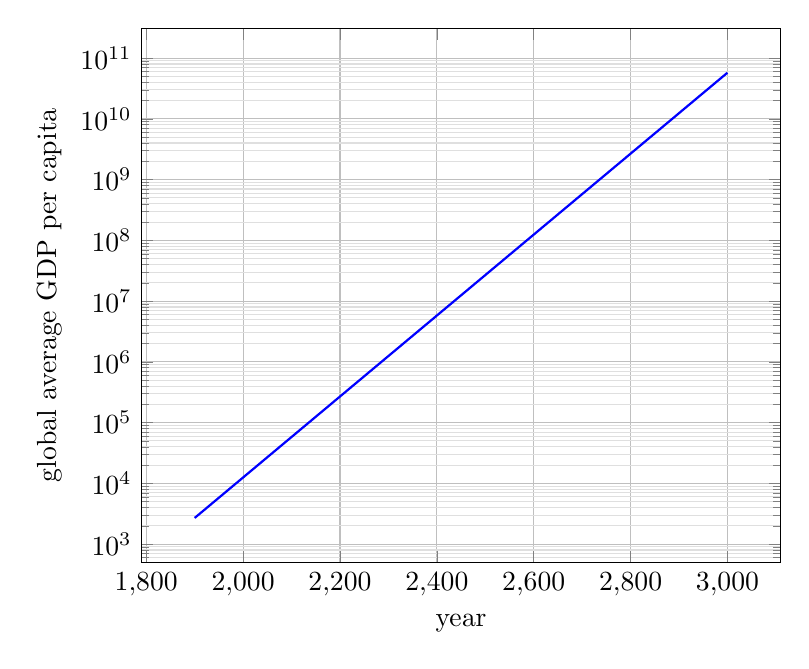
\begin{tikzpicture}
		\begin{axis}[
			width=0.8\linewidth,
			xlabel=year,
			ylabel=global average GDP per capita,
			ymode=log,
			%xmin=1, xmax=100,
			%ymin=0, ymax=10,
			grid=both,
			minor grid style={gray!25},
			major grid style={gray!50},
			]
			\addplot[blue, thick, domain=1900:3000, samples=100]  {2700*pow(1.015450028,x-1900)};
		\end{axis}
	\end{tikzpicture}
	
	Here are some precise numbers to be extracted from this:
	
	(once again, in international dollars, at 2017 prices)
	
	\begin{center}
		\begin{tabular}{c | c | c | c }
		year & exact GDP p.c. & rough GDP p.c. & order of magnitude \\\hline
		2000 & 12 508.9 \$ & $12.5\times10^3$ \$ & tens of thousands \\\hline
		2050 & 26 924.47 \$ & $26.9\times10^3$ \$ & tens of thousands \\\hline
		2100 & 57 952.87 \$ & $58\times10^3$ \$ & tens of thousands \\\hline
		2150 & 124 739.13 \$ & $124.7\times10^3$ \$ & hundreds of thousands \\\hline
		2200 & 268 491.49 \$ & $268.5\times10^3$ \$ & hundreds of thousands \\\hline
		2250 & 577 907.5 \$ & $577.9\times10^3$ \$ & hundreds of thousands \\\hline
		2300 & 1 243 901.89 \$ & $1.2\times10^6$ \$ & millions \\\hline
		2350 & 2 677 404.09 \$ & $2.7\times10^6$ \$ & millions \\\hline
		2400 & 5 762 908.41 \$ & $5.8\times10^6$ \$ & millions \\\hline
		2450 & 12 404 221.5 \$ & $12.4\times10^6$ \$ & tens of millions \\\hline
		2500 & 26 699 142.17 \$ & $26.7\times10^6$ \$ & tens of millions \\\hline
		2600 & 123 695 214.67 \$ & $123.7\times10^6$ \$ & hundreds of millions \\\hline
		2700 & 573 071 075.94 \$ & $573\times10^6$ \$ & hundreds of millions \\\hline
		2800 & 2 654 997 276.55 \$ & $2.7\times10^9$ \$ & billions \\\hline
		2900 & 12 300 412 347.57 \$ & $12.3\times10^9$ \$ & tens of billions \\\hline
		3000 & 56 986 929 989.15 \$ & $57\times10^9$ \$ & tens of billions \\
		\end{tabular}
	\end{center}
	
	\pagebreak
	
	\small
	
	\noindent
	\begin{tabular}{|c|c|}
		\hline
		year & GDP p.c. \\
		\hline
		2025 & 1.8352E+04 \\
		\hline
		2030 & 1.9814E+04 \\
		\hline
		2035 & 2.1393E+04 \\
		\hline
		2040 & 2.3097E+04 \\
		\hline
		2045 & 2.4938E+04 \\
		\hline
		2050 & 2.6924E+04 \\
		\hline
		2055 & 2.9070E+04 \\
		\hline
		2060 & 3.1386E+04 \\
		\hline
		2065 & 3.3886E+04 \\
		\hline
		2070 & 3.6586E+04 \\
		\hline
		2075 & 3.9501E+04 \\
		\hline
		2080 & 4.2649E+04 \\
		\hline
		2085 & 4.6046E+04 \\
		\hline
		2090 & 4.9715E+04 \\
		\hline
		2095 & 5.3676E+04 \\
		\hline
		2100 & 5.7953E+04 \\
		\hline
		2105 & 6.2570E+04 \\
		\hline
		2110 & 6.7555E+04 \\
		\hline
		2115 & 7.2938E+04 \\
		\hline
		2120 & 7.8749E+04 \\
		\hline
		2125 & 8.5023E+04 \\
		\hline
		2130 & 9.1798E+04 \\
		\hline
		2135 & 9.9112E+04 \\
		\hline
		2140 & 1.0701E+05 \\
		\hline
		2145 & 1.1553E+05 \\
		\hline
		2150 & 1.2474E+05 \\
		\hline
		2155 & 1.3468E+05 \\
		\hline
		2160 & 1.4541E+05 \\
		\hline
		2165 & 1.5699E+05 \\
		\hline
		2170 & 1.6950E+05 \\
		\hline
		2175 & 1.8301E+05 \\
		\hline
		2180 & 1.9759E+05 \\
		\hline
		2185 & 2.1333E+05 \\
		\hline
		2190 & 2.3033E+05 \\
		\hline
		2195 & 2.4868E+05 \\
		\hline
		2200 & 2.6849E+05 \\
		\hline
		2205 & 2.8988E+05 \\
		\hline
		2210 & 3.1298E+05 \\
		\hline
		2215 & 3.3792E+05 \\
		\hline
		2220 & 3.6484E+05 \\
		\hline
		2225 & 3.9391E+05 \\
		\hline
		2230 & 4.2529E+05 \\
		\hline
		2235 & 4.5918E+05 \\
		\hline
		2240 & 4.9576E+05 \\
		\hline
		2245 & 5.3526E+05 \\
		\hline
		2250 & 5.7791E+05 \\
		\hline
		2255 & 6.2395E+05 \\
		\hline
		2260 & 6.7366E+05 \\
		\hline
		2265 & 7.2734E+05 \\
		\hline
	\end{tabular}
	\hfill
	\begin{tabular}{|c|c|}
		\hline
		year & GDP p.c. \\
		\hline
		2270 & 7.8529E+05 \\
		\hline
		2275 & 8.4786E+05 \\
		\hline
		2280 & 9.1541E+05 \\
		\hline
		2285 & 9.8834E+05 \\
		\hline
		2290 & 1.0671E+06 \\
		\hline
		2295 & 1.1521E+06 \\
		\hline
		2300 & 1.2439E+06 \\
		\hline
		2305 & 1.3430E+06 \\
		\hline
		2310 & 1.4500E+06 \\
		\hline
		2315 & 1.5655E+06 \\
		\hline
		2320 & 1.6903E+06 \\
		\hline
		2325 & 1.8249E+06 \\
		\hline
		2330 & 1.9703E+06 \\
		\hline
		2335 & 2.1273E+06 \\
		\hline
		2340 & 2.2968E+06 \\
		\hline
		2345 & 2.4798E+06 \\
		\hline
		2350 & 2.6774E+06 \\
		\hline
		2355 & 2.8907E+06 \\
		\hline
		2360 & 3.1210E+06 \\
		\hline
		2365 & 3.3697E+06 \\
		\hline
		2370 & 3.6382E+06 \\
		\hline
		2375 & 3.9281E+06 \\
		\hline
		2380 & 4.2410E+06 \\
		\hline
		2385 & 4.5789E+06 \\
		\hline
		2390 & 4.9437E+06 \\
		\hline
		2395 & 5.3376E+06 \\
		\hline
		2400 & 5.7629E+06 \\
		\hline
		2405 & 6.2221E+06 \\
		\hline
		2410 & 6.7178E+06 \\
		\hline
		2415 & 7.2530E+06 \\
		\hline
		2420 & 7.8309E+06 \\
		\hline
		2425 & 8.4548E+06 \\
		\hline
		2430 & 9.1285E+06 \\
		\hline
		2435 & 9.8558E+06 \\
		\hline
		2440 & 1.0641E+07 \\
		\hline
		2445 & 1.1489E+07 \\
		\hline
		2450 & 1.2404E+07 \\
		\hline
		2455 & 1.3393E+07 \\
		\hline
		2460 & 1.4460E+07 \\
		\hline
		2465 & 1.5612E+07 \\
		\hline
		2470 & 1.6855E+07 \\
		\hline
		2475 & 1.8198E+07 \\
		\hline
		2480 & 1.9648E+07 \\
		\hline
		2485 & 2.1214E+07 \\
		\hline
		2490 & 2.2904E+07 \\
		\hline
		2495 & 2.4729E+07 \\
		\hline
		2500 & 2.6699E+07 \\
		\hline
		2505 & 2.8826E+07 \\
		\hline
		2510 & 3.1123E+07 \\
		\hline
	\end{tabular}
	\hfill
	\begin{tabular}{|c|c|}
		\hline
		year & GDP p.c. \\
		\hline
		2515 & 3.3603E+07 \\
		\hline
		2520 & 3.6280E+07 \\
		\hline
		2525 & 3.9171E+07 \\
		\hline
		2530 & 4.2292E+07 \\
		\hline
		2535 & 4.5661E+07 \\
		\hline
		2540 & 4.9299E+07 \\
		\hline
		2545 & 5.3227E+07 \\
		\hline
		2550 & 5.7468E+07 \\
		\hline
		2555 & 6.2047E+07 \\
		\hline
		2560 & 6.6990E+07 \\
		\hline
		2565 & 7.2327E+07 \\
		\hline
		2570 & 7.8090E+07 \\
		\hline
		2575 & 8.4312E+07 \\
		\hline
		2580 & 9.1029E+07 \\
		\hline
		2585 & 9.8282E+07 \\
		\hline
		2590 & 1.0611E+08 \\
		\hline
		2595 & 1.1457E+08 \\
		\hline
		2600 & 1.2370E+08 \\
		\hline
		2605 & 1.3355E+08 \\
		\hline
		2610 & 1.4419E+08 \\
		\hline
		2615 & 1.5568E+08 \\
		\hline
		2620 & 1.6808E+08 \\
		\hline
		2625 & 1.8147E+08 \\
		\hline
		2630 & 1.9593E+08 \\
		\hline
		2635 & 2.1154E+08 \\
		\hline
		2640 & 2.2840E+08 \\
		\hline
		2645 & 2.4660E+08 \\
		\hline
		2650 & 2.6624E+08 \\
		\hline
		2655 & 2.8746E+08 \\
		\hline
		2660 & 3.1036E+08 \\
		\hline
		2665 & 3.3509E+08 \\
		\hline
		2670 & 3.6179E+08 \\
		\hline
		2675 & 3.9061E+08 \\
		\hline
		2680 & 4.2173E+08 \\
		\hline
		2685 & 4.5533E+08 \\
		\hline
		2690 & 4.9161E+08 \\
		\hline
		2695 & 5.3078E+08 \\
		\hline
		2700 & 5.7307E+08 \\
		\hline
		2705 & 6.1873E+08 \\
		\hline
		2710 & 6.6803E+08 \\
		\hline
		2715 & 7.2125E+08 \\
		\hline
		2720 & 7.7872E+08 \\
		\hline
		2725 & 8.4076E+08 \\
		\hline
		2730 & 9.0775E+08 \\
		\hline
		2735 & 9.8007E+08 \\
		\hline
		2740 & 1.0582E+09 \\
		\hline
		2745 & 1.1425E+09 \\
		\hline
		2750 & 1.2335E+09 \\
		\hline
		2755 & 1.3318E+09 \\
		\hline
	\end{tabular}
	\hfill
	\begin{tabular}{|c|c|}
		\hline
		year & GDP p.c. \\
		\hline
		2760 & 1.4379E+09 \\
		\hline
		2765 & 1.5524E+09 \\
		\hline
		2770 & 1.6761E+09 \\
		\hline
		2775 & 1.8097E+09 \\
		\hline
		2780 & 1.9539E+09 \\
		\hline
		2785 & 2.1095E+09 \\
		\hline
		2790 & 2.2776E+09 \\
		\hline
		2795 & 2.4591E+09 \\
		\hline
		2800 & 2.6550E+09 \\
		\hline
		2805 & 2.8665E+09 \\
		\hline
		2810 & 3.0949E+09 \\
		\hline
		2815 & 3.3415E+09 \\
		\hline
		2820 & 3.6077E+09 \\
		\hline
		2825 & 3.8952E+09 \\
		\hline
		2830 & 4.2055E+09 \\
		\hline
		2835 & 4.5406E+09 \\
		\hline
		2840 & 4.9024E+09 \\
		\hline
		2845 & 5.2930E+09 \\
		\hline
		2850 & 5.7147E+09 \\
		\hline
		2855 & 6.1700E+09 \\
		\hline
		2860 & 6.6616E+09 \\
		\hline
		2865 & 7.1923E+09 \\
		\hline
		2870 & 7.7654E+09 \\
		\hline
		2875 & 8.3841E+09 \\
		\hline
		2880 & 9.0521E+09 \\
		\hline
		2885 & 9.7733E+09 \\
		\hline
		2890 & 1.0552E+10 \\
		\hline
		2895 & 1.1393E+10 \\
		\hline
		2900 & 1.2300E+10 \\
		\hline
		2905 & 1.3280E+10 \\
		\hline
		2910 & 1.4339E+10 \\
		\hline
		2915 & 1.5481E+10 \\
		\hline
		2920 & 1.6714E+10 \\
		\hline
		2925 & 1.8046E+10 \\
		\hline
		2930 & 1.9484E+10 \\
		\hline
		2935 & 2.1036E+10 \\
		\hline
		2940 & 2.2712E+10 \\
		\hline
		2945 & 2.4522E+10 \\
		\hline
		2950 & 2.6476E+10 \\
		\hline
		2955 & 2.8585E+10 \\
		\hline
		2960 & 3.0863E+10 \\
		\hline
		2965 & 3.3322E+10 \\
		\hline
		2970 & 3.5976E+10 \\
		\hline
		2975 & 3.8843E+10 \\
		\hline
		2980 & 4.1938E+10 \\
		\hline
		2985 & 4.5279E+10 \\
		\hline
		2990 & 4.8887E+10 \\
		\hline
		2995 & 5.2782E+10 \\
		\hline
		3000 & 5.6987E+10 \\
		\hline
	\end{tabular}
	
	\normalsize
	
	\pagebreak
	
	\section{exponential global total GDP}
	
	As mentioned in the previous section, given the population growth and average GDP per capita growth rates, the total GDP growth rate is expected to be 2.88\% per year.
	
	\medskip
	
	Below in red I've ploted the global total GDP (expressed in international dollars at 2017 prices) between years 1900 and 2022 according to Our World In Data, and in blue an exponential function:
	
	\begin{center}
		{\large $ y = 4188242000000 \times 1.029144185^{x-1900} $}
	\end{center}
	
	\noindent Which represents a starting point at year 1900 with 4188242000000 international-\$, and growth of roughly 2.91\% per year.
	
	\bigskip
	
	Additionally I've plotted in green the function mentioned previously which I deduced from the population and GDP per capita growth:
	
	\begin{center}
		{\large $ y = 4188242000000 \times 1.028803019^{x-1900} $}
	\end{center}

	\noindent Which represents growth at 2.88\% per year from the same starting point.
	
	\medskip
	
	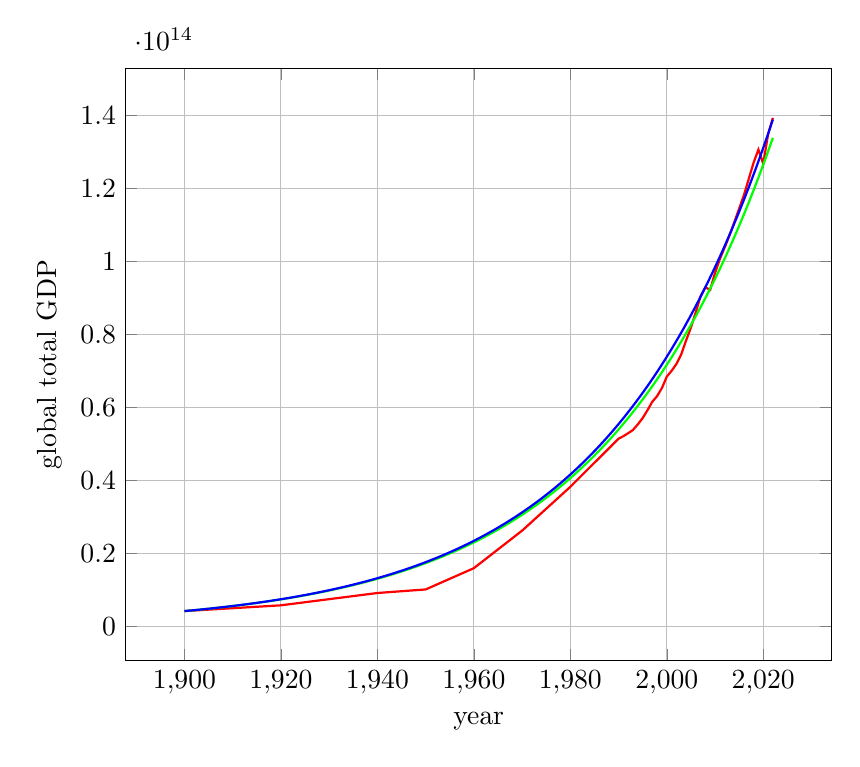
\begin{tikzpicture}
		\begin{axis}[
			width=0.87\linewidth,
			xlabel=year,
			ylabel=global total GDP,
			%ymode=log,
			%xmin=1, xmax=100,
			%ymin=0, ymax=10,
			grid=both,
			minor grid style={gray!25},
			major grid style={gray!50},
			]
			\addplot[red, thick] coordinates {
				(1900,4188242000000)
				(1920,5767619000000)
				(1940,9140895000000)
				(1950,10114720000000)
				(1960,15943992000000)
				(1970,26228820000000)
				(1980,38231190000000)
				(1990,51441260000000)
				(1991,52114010000000)
				(1992,52945970000000)
				(1993,53832466000000)
				(1994,55357636000000)
				(1995,57087963000000)
				(1996,59237120000000)
				(1997,61557950000000)
				(1998,63106750000000)
				(1999,65330135000000)
				(2000,68437053000000)
				(2001,70024640000000)
				(2002,71903790000000)
				(2003,74554945000000)
				(2004,78333000000000)
				(2005,81878480000000)
				(2006,86054376000000)
				(2007,90450730000000)
				(2008,92899120000000)
				(2009,92208030000000)
				(2010,96879270000000)
				(2011,100612600000000)
				(2012,103806240000000)
				(2013,107140240000000)
				(2014,110775960000000)
				(2015,114471780000000)
				(2016,118180714000000)
				(2017,122635850000000)
				(2018,127074744000000)
				(2019,130661590000000)
				(2020,126791940000000)
				(2021,134821810000000)
				(2022,139357755000000)
			};
			\addplot[green, thick, domain=1900:2022, samples=100]  {4188242000000*pow(1.028803019,x-1900)};
			\addplot[blue, thick, domain=1900:2022, samples=100]  {4188242000000*pow(1.029144185,x-1900)};
		\end{axis}
	\end{tikzpicture}
	
	\medskip
	
	As can be seen, the data is consistent with previous predictions. The blue curve intersects the final point of the data here (year 2022) as it should given how it is calculated, while the green deduced from population and gdp per capita data intersects the point for 2021 year, possibly reflecting the fact my data for global average gdp per capita runs from 1900 to 2021 and not 2022.
	
	\pagebreak
	
	Let's extrapolate the found rates of growth - both 2.88\% and 2.91\% - all the way to the year 3000. First, \textbf{2.88\%} which is the rate consistent with GDP per capita \& population growth shown earlier:
	
	\medskip
	
	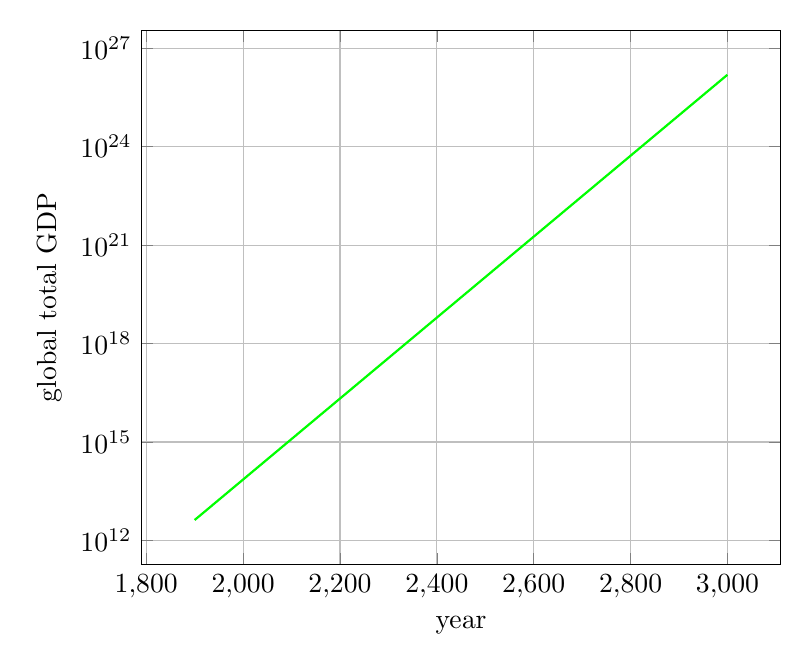
\begin{tikzpicture}
		\begin{axis}[
			width=0.8\linewidth,
			xlabel=year,
			ylabel=global total GDP,
			ymode=log,
			%xmin=1, xmax=100,
			%ymin=0, ymax=10,
			grid=both,
			minor grid style={gray!25},
			major grid style={gray!50},
			]
			\addplot[green, thick, domain=1900:3000, samples=100]  {4188242000000*pow(1.028803019,x-1900)};
		\end{axis}
	\end{tikzpicture}

	Here are the numbers that can be extracted from this:
	
	\begin{center}
		\begin{tabular}{c | c | c }
			year & exact GDP (exp. 2.88\%) & rough \\\hline
			2000 & 71 656 364 205 474 \$ & 7.17$\times10^{13}$ \$  \\\hline
			2050 & 296 391 857 890 027 \$ & 2.96$\times10^{14}$ \$  \\\hline
			2100 & 1 225 964 147 044 890 \$ & 1.23$\times10^{15}$ \$  \\\hline
			2150 & 5 070 949 318 712 950 \$ & 5.07$\times10^{15}$ \$  \\\hline
			2200 & 20 974 942 093 485 100 \$ & 2.10$\times10^{16}$ \$  \\\hline
			2250 & 86 758 547 201 713 000 \$ & 8.68$\times10^{16}$ \$  \\\hline
			2300 & 358 858 941 254 946 000 \$ & 3.59$\times10^{17}$ \$  \\\hline
			2350 & 1 484 346 428 936 960 000 \$ & 1.48$\times10^{18}$ \$  \\\hline
			2400 & 6 139 694 648 245 090 000 \$ & 6.14$\times10^{18}$ \$  \\\hline
			2450 & 25 395 588 010 196 600 000 \$ & 2.54$\times10^{19}$ \$  \\\hline
			2500 & 105 043 642 613 071 000 000 \$ & 1.05$\times10^{20}$ \$  \\\hline
			2600 & 1 797 184 955 537 870 000 000 \$ & 1.80$\times10^{21}$ \$  \\\hline
			2700 & 30 747 922 330 806 300 000 000 \$ & 3.07$\times10^{22}$ \$  \\\hline
			2800 & 526 064 234 372 774 000 000 000 \$ & 5.26$\times10^{23}$ \$  \\\hline
			2900 & 9 000 399 302 067 420 000 000 000 \$ & 9.00$\times10^{24}$ \$  \\\hline
			3000 & 153 987 255 364 814 000 000 000 000 \$ & 1.54$\times10^{26}$ \$
		\end{tabular}
	\end{center}
	
	\pagebreak
	
	\small
	
	\noindent
	\begin{tabular}{|c|c|}
		\hline
		year & GDP (2.88\%) \\
		\hline
		2025 & 1.4573E+14 \\
		\hline
		2030 & 1.6797E+14 \\
		\hline
		2035 & 1.9359E+14 \\
		\hline
		2040 & 2.2312E+14 \\
		\hline
		2045 & 2.5716E+14 \\
		\hline
		2050 & 2.9639E+14 \\
		\hline
		2055 & 3.4161E+14 \\
		\hline
		2060 & 3.9372E+14 \\
		\hline
		2065 & 4.5378E+14 \\
		\hline
		2070 & 5.2301E+14 \\
		\hline
		2075 & 6.0280E+14 \\
		\hline
		2080 & 6.9476E+14 \\
		\hline
		2085 & 8.0075E+14 \\
		\hline
		2090 & 9.2290E+14 \\
		\hline
		2095 & 1.0637E+15 \\
		\hline
		2100 & 1.2260E+15 \\
		\hline
		2105 & 1.4130E+15 \\
		\hline
		2110 & 1.6285E+15 \\
		\hline
		2115 & 1.8770E+15 \\
		\hline
		2120 & 2.1633E+15 \\
		\hline
		2125 & 2.4934E+15 \\
		\hline
		2130 & 2.8737E+15 \\
		\hline
		2135 & 3.3121E+15 \\
		\hline
		2140 & 3.8174E+15 \\
		\hline
		2145 & 4.3998E+15 \\
		\hline
		2150 & 5.0709E+15 \\
		\hline
		2155 & 5.8445E+15 \\
		\hline
		2160 & 6.7361E+15 \\
		\hline
		2165 & 7.7638E+15 \\
		\hline
		2170 & 8.9482E+15 \\
		\hline
		2175 & 1.0313E+16 \\
		\hline
		2180 & 1.1887E+16 \\
		\hline
		2185 & 1.3700E+16 \\
		\hline
		2190 & 1.5790E+16 \\
		\hline
		2195 & 1.8199E+16 \\
		\hline
		2200 & 2.0975E+16 \\
		\hline
		2205 & 2.4175E+16 \\
		\hline
		2210 & 2.7863E+16 \\
		\hline
		2215 & 3.2113E+16 \\
		\hline
		2220 & 3.7012E+16 \\
		\hline
		2225 & 4.2659E+16 \\
		\hline
		2230 & 4.9166E+16 \\
		\hline
		2235 & 5.6667E+16 \\
		\hline
		2240 & 6.5312E+16 \\
		\hline
		2245 & 7.5275E+16 \\
		\hline
		2250 & 8.6759E+16 \\
		\hline
		2255 & 9.9994E+16 \\
		\hline
		2260 & 1.1525E+17 \\
		\hline
		2265 & 1.3283E+17 \\
		\hline
	\end{tabular}
	\hfill
	\begin{tabular}{|c|c|}
		\hline
		year & GDP (2.88\%) \\
		\hline
		2270 & 1.5309E+17 \\
		\hline
		2275 & 1.7645E+17 \\
		\hline
		2280 & 2.0337E+17 \\
		\hline
		2285 & 2.3439E+17 \\
		\hline
		2290 & 2.7015E+17 \\
		\hline
		2295 & 3.1136E+17 \\
		\hline
		2300 & 3.5886E+17 \\
		\hline
		2305 & 4.1360E+17 \\
		\hline
		2310 & 4.7670E+17 \\
		\hline
		2315 & 5.4942E+17 \\
		\hline
		2320 & 6.3324E+17 \\
		\hline
		2325 & 7.2984E+17 \\
		\hline
		2330 & 8.4118E+17 \\
		\hline
		2335 & 9.6951E+17 \\
		\hline
		2340 & 1.1174E+18 \\
		\hline
		2345 & 1.2879E+18 \\
		\hline
		2350 & 1.4843E+18 \\
		\hline
		2355 & 1.7108E+18 \\
		\hline
		2360 & 1.9718E+18 \\
		\hline
		2365 & 2.2726E+18 \\
		\hline
		2370 & 2.6193E+18 \\
		\hline
		2375 & 3.0188E+18 \\
		\hline
		2380 & 3.4794E+18 \\
		\hline
		2385 & 4.0102E+18 \\
		\hline
		2390 & 4.6219E+18 \\
		\hline
		2395 & 5.3270E+18 \\
		\hline
		2400 & 6.1397E+18 \\
		\hline
		2405 & 7.0763E+18 \\
		\hline
		2410 & 8.1558E+18 \\
		\hline
		2415 & 9.4001E+18 \\
		\hline
		2420 & 1.0834E+19 \\
		\hline
		2425 & 1.2487E+19 \\
		\hline
		2430 & 1.4392E+19 \\
		\hline
		2435 & 1.6587E+19 \\
		\hline
		2440 & 1.9118E+19 \\
		\hline
		2445 & 2.2034E+19 \\
		\hline
		2450 & 2.5396E+19 \\
		\hline
		2455 & 2.9270E+19 \\
		\hline
		2460 & 3.3735E+19 \\
		\hline
		2465 & 3.8881E+19 \\
		\hline
		2470 & 4.4813E+19 \\
		\hline
		2475 & 5.1649E+19 \\
		\hline
		2480 & 5.9529E+19 \\
		\hline
		2485 & 6.8610E+19 \\
		\hline
		2490 & 7.9077E+19 \\
		\hline
		2495 & 9.1140E+19 \\
		\hline
		2500 & 1.0504E+20 \\
		\hline
		2505 & 1.2107E+20 \\
		\hline
		2510 & 1.3954E+20 \\
		\hline
	\end{tabular}
	\hfill
	\begin{tabular}{|c|c|}
		\hline
		year & GDP (2.88\%) \\
		\hline
		2515 & 1.6082E+20 \\
		\hline
		2520 & 1.8536E+20 \\
		\hline
		2525 & 2.1364E+20 \\
		\hline
		2530 & 2.4623E+20 \\
		\hline
		2535 & 2.8379E+20 \\
		\hline
		2540 & 3.2708E+20 \\
		\hline
		2545 & 3.7698E+20 \\
		\hline
		2550 & 4.3449E+20 \\
		\hline
		2555 & 5.0077E+20 \\
		\hline
		2560 & 5.7717E+20 \\
		\hline
		2565 & 6.6522E+20 \\
		\hline
		2570 & 7.6670E+20 \\
		\hline
		2575 & 8.8366E+20 \\
		\hline
		2580 & 1.0185E+21 \\
		\hline
		2585 & 1.1738E+21 \\
		\hline
		2590 & 1.3529E+21 \\
		\hline
		2595 & 1.5593E+21 \\
		\hline
		2600 & 1.7972E+21 \\
		\hline
		2605 & 2.0714E+21 \\
		\hline
		2610 & 2.3873E+21 \\
		\hline
		2615 & 2.7515E+21 \\
		\hline
		2620 & 3.1713E+21 \\
		\hline
		2625 & 3.6551E+21 \\
		\hline
		2630 & 4.2127E+21 \\
		\hline
		2635 & 4.8554E+21 \\
		\hline
		2640 & 5.5961E+21 \\
		\hline
		2645 & 6.4498E+21 \\
		\hline
		2650 & 7.4337E+21 \\
		\hline
		2655 & 8.5677E+21 \\
		\hline
		2660 & 9.8748E+21 \\
		\hline
		2665 & 1.1381E+22 \\
		\hline
		2670 & 1.3117E+22 \\
		\hline
		2675 & 1.5119E+22 \\
		\hline
		2680 & 1.7425E+22 \\
		\hline
		2685 & 2.0083E+22 \\
		\hline
		2690 & 2.3147E+22 \\
		\hline
		2695 & 2.6678E+22 \\
		\hline
		2700 & 3.0748E+22 \\
		\hline
		2705 & 3.5439E+22 \\
		\hline
		2710 & 4.0845E+22 \\
		\hline
		2715 & 4.7076E+22 \\
		\hline
		2720 & 5.4258E+22 \\
		\hline
		2725 & 6.2535E+22 \\
		\hline
		2730 & 7.2075E+22 \\
		\hline
		2735 & 8.3070E+22 \\
		\hline
		2740 & 9.5743E+22 \\
		\hline
		2745 & 1.1035E+23 \\
		\hline
		2750 & 1.2718E+23 \\
		\hline
		2755 & 1.4658E+23 \\
		\hline
	\end{tabular}
	\hfill
	\begin{tabular}{|c|c|}
		\hline
		year & GDP (2.88\%) \\
		\hline
		2760 & 1.6895E+23 \\
		\hline
		2765 & 1.9472E+23 \\
		\hline
		2770 & 2.2443E+23 \\
		\hline
		2775 & 2.5866E+23 \\
		\hline
		2780 & 2.9812E+23 \\
		\hline
		2785 & 3.4360E+23 \\
		\hline
		2790 & 3.9602E+23 \\
		\hline
		2795 & 4.5643E+23 \\
		\hline
		2800 & 5.2606E+23 \\
		\hline
		2805 & 6.0632E+23 \\
		\hline
		2810 & 6.9881E+23 \\
		\hline
		2815 & 8.0542E+23 \\
		\hline
		2820 & 9.2829E+23 \\
		\hline
		2825 & 1.0699E+24 \\
		\hline
		2830 & 1.2331E+24 \\
		\hline
		2835 & 1.4212E+24 \\
		\hline
		2840 & 1.6381E+24 \\
		\hline
		2845 & 1.8879E+24 \\
		\hline
		2850 & 2.1760E+24 \\
		\hline
		2855 & 2.5079E+24 \\
		\hline
		2860 & 2.8905E+24 \\
		\hline
		2865 & 3.3315E+24 \\
		\hline
		2870 & 3.8397E+24 \\
		\hline
		2875 & 4.4254E+24 \\
		\hline
		2880 & 5.1006E+24 \\
		\hline
		2885 & 5.8787E+24 \\
		\hline
		2890 & 6.7755E+24 \\
		\hline
		2895 & 7.8091E+24 \\
		\hline
		2900 & 9.0004E+24 \\
		\hline
		2905 & 1.0373E+25 \\
		\hline
		2910 & 1.1956E+25 \\
		\hline
		2915 & 1.3780E+25 \\
		\hline
		2920 & 1.5882E+25 \\
		\hline
		2925 & 1.8305E+25 \\
		\hline
		2930 & 2.1097E+25 \\
		\hline
		2935 & 2.4316E+25 \\
		\hline
		2940 & 2.8025E+25 \\
		\hline
		2945 & 3.2301E+25 \\
		\hline
		2950 & 3.7228E+25 \\
		\hline
		2955 & 4.2908E+25 \\
		\hline
		2960 & 4.9453E+25 \\
		\hline
		2965 & 5.6998E+25 \\
		\hline
		2970 & 6.5693E+25 \\
		\hline
		2975 & 7.5714E+25 \\
		\hline
		2980 & 8.7265E+25 \\
		\hline
		2985 & 1.0058E+26 \\
		\hline
		2990 & 1.1592E+26 \\
		\hline
		2995 & 1.3361E+26 \\
		\hline
		3000 & 1.5399E+26 \\
		\hline
	\end{tabular}
	
	\normalsize
	
	\pagebreak
	
	Now again, for \textbf{2.91\%} which is the rate deduced from the actual data for global total gdp gathered from Our World In Data:
	
	\medskip
	
	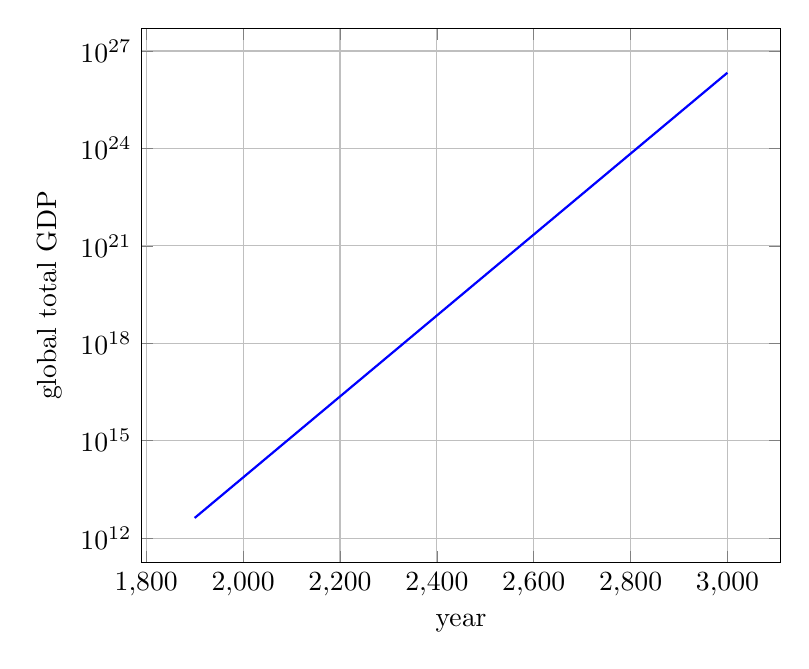
\begin{tikzpicture}
		\begin{axis}[
			width=0.8\linewidth,
			xlabel=year,
			ylabel=global total GDP,
			ymode=log,
			%xmin=1, xmax=100,
			%ymin=0, ymax=10,
			grid=both,
			minor grid style={gray!25},
			major grid style={gray!50},
			]
			\addplot[blue, thick, domain=1900:3000, samples=100]  {4188242000000*pow(1.029144185,x-1900)};
		\end{axis}
	\end{tikzpicture}
	
	Here are the numbers that can be extracted from this:
	
	\begin{center}
		\begin{tabular}{c | c | c }
			year & exact GDP (exp. 2.91\%) & rough \\\hline
			2000 & 74 072 024 713 093 \$ & 7.41$\times10^{13}$ \$ \\\hline
			2050 & 311 505 299 969 375 \$ & 3.12$\times10^{14}$ \$ \\\hline
			2100 & 1 310 016 194 168 611 \$ & 1.31$\times10^{15}$ \$ \\\hline
			2150 & 5 509 191 750 999 848 \$ & 5.51$\times10^{15}$ \$ \\\hline
			2200 & 23 168 563 781 417 100 \$ & 2.32$\times10^{16}$ \$ \\\hline
			2250 & 97 433 956 187 161 900 \$ & 9.74$\times10^{16}$ \$ \\\hline
			2300 & 409 752 451 979 616 000 \$ & 4.10$\times10^{17}$ \$ \\\hline
			2350 & 1 723 188 490 681 750 000 \$ & 1.72$\times10^{18}$ \$ \\\hline
			2400 & 7 246 762 185 490 900 000 \$ & 7.25$\times10^{18}$ \$ \\\hline
			2450 & 30 475 808 338 462 100 000 \$ & 3.05$\times10^{19}$ \$ \\\hline
			2500 & 128 164 119 383 167 000 000 \$ & 1.28$\times10^{20}$ \$ \\\hline
			2600 & 2 266 673 181 320 900 000 000 \$ & 2.27$\times10^{21}$ \$ \\\hline
			2700 & 40 087 719 836 463 000 000 000 \$ & 4.01$\times10^{22}$ \$ \\\hline
			2800 & 708 979 704 233 437 000 000 000 \$ & 7.09$\times10^{23}$ \$ \\\hline
			2900 & 12 538 807 970 757 400 000 000 000 \$ & 1.25$\times10^{25}$ \$ \\\hline
			3000 & 221 757 695 444 216 000 000 000 000 \$ & 2.22$\times10^{26}$ \$
		\end{tabular}
	\end{center}
	
	\pagebreak
	
	\small
	
	\noindent
	\begin{tabular}{|c|c|}
		\hline
		year & GDP (2.91\%) \\
		\hline
		2025 & 1.5190E+14 \\
		\hline
		2030 & 1.7536E+14 \\
		\hline
		2035 & 2.0245E+14 \\
		\hline
		2040 & 2.3372E+14 \\
		\hline
		2045 & 2.6983E+14 \\
		\hline
		2050 & 3.1151E+14 \\
		\hline
		2055 & 3.5962E+14 \\
		\hline
		2060 & 4.1517E+14 \\
		\hline
		2065 & 4.7930E+14 \\
		\hline
		2070 & 5.5334E+14 \\
		\hline
		2075 & 6.3881E+14 \\
		\hline
		2080 & 7.3748E+14 \\
		\hline
		2085 & 8.5140E+14 \\
		\hline
		2090 & 9.8291E+14 \\
		\hline
		2095 & 1.1347E+15 \\
		\hline
		2100 & 1.3100E+15 \\
		\hline
		2105 & 1.5124E+15 \\
		\hline
		2110 & 1.7460E+15 \\
		\hline
		2115 & 2.0157E+15 \\
		\hline
		2120 & 2.3270E+15 \\
		\hline
		2125 & 2.6865E+15 \\
		\hline
		2130 & 3.1014E+15 \\
		\hline
		2135 & 3.5805E+15 \\
		\hline
		2140 & 4.1336E+15 \\
		\hline
		2145 & 4.7721E+15 \\
		\hline
		2150 & 5.5092E+15 \\
		\hline
		2155 & 6.3602E+15 \\
		\hline
		2160 & 7.3426E+15 \\
		\hline
		2165 & 8.4768E+15 \\
		\hline
		2170 & 9.7862E+15 \\
		\hline
		2175 & 1.1298E+16 \\
		\hline
		2180 & 1.3043E+16 \\
		\hline
		2185 & 1.5058E+16 \\
		\hline
		2190 & 1.7383E+16 \\
		\hline
		2195 & 2.0069E+16 \\
		\hline
		2200 & 2.3169E+16 \\
		\hline
		2205 & 2.6747E+16 \\
		\hline
		2210 & 3.0879E+16 \\
		\hline
		2215 & 3.5649E+16 \\
		\hline
		2220 & 4.1155E+16 \\
		\hline
		2225 & 4.7512E+16 \\
		\hline
		2230 & 5.4851E+16 \\
		\hline
		2235 & 6.3324E+16 \\
		\hline
		2240 & 7.3105E+16 \\
		\hline
		2245 & 8.4397E+16 \\
		\hline
		2250 & 9.7434E+16 \\
		\hline
		2255 & 1.1248E+17 \\
		\hline
		2260 & 1.2986E+17 \\
		\hline
		2265 & 1.4992E+17 \\
		\hline
	\end{tabular}
	\hfill
	\begin{tabular}{|c|c|}
		\hline
		year & GDP (2.91\%) \\
		\hline
		2270 & 1.7308E+17 \\
		\hline
		2275 & 1.9981E+17 \\
		\hline
		2280 & 2.3067E+17 \\
		\hline
		2285 & 2.6630E+17 \\
		\hline
		2290 & 3.0744E+17 \\
		\hline
		2295 & 3.5493E+17 \\
		\hline
		2300 & 4.0975E+17 \\
		\hline
		2305 & 4.7305E+17 \\
		\hline
		2310 & 5.4611E+17 \\
		\hline
		2315 & 6.3047E+17 \\
		\hline
		2320 & 7.2786E+17 \\
		\hline
		2325 & 8.4029E+17 \\
		\hline
		2330 & 9.7008E+17 \\
		\hline
		2335 & 1.1199E+18 \\
		\hline
		2340 & 1.2929E+18 \\
		\hline
		2345 & 1.4926E+18 \\
		\hline
		2350 & 1.7232E+18 \\
		\hline
		2355 & 1.9894E+18 \\
		\hline
		2360 & 2.2967E+18 \\
		\hline
		2365 & 2.6514E+18 \\
		\hline
		2370 & 3.0610E+18 \\
		\hline
		2375 & 3.5338E+18 \\
		\hline
		2380 & 4.0796E+18 \\
		\hline
		2385 & 4.7098E+18 \\
		\hline
		2390 & 5.4373E+18 \\
		\hline
		2395 & 6.2772E+18 \\
		\hline
		2400 & 7.2468E+18 \\
		\hline
		2405 & 8.3661E+18 \\
		\hline
		2410 & 9.6584E+18 \\
		\hline
		2415 & 1.1150E+19 \\
		\hline
		2420 & 1.2873E+19 \\
		\hline
		2425 & 1.4861E+19 \\
		\hline
		2430 & 1.7157E+19 \\
		\hline
		2435 & 1.9807E+19 \\
		\hline
		2440 & 2.2866E+19 \\
		\hline
		2445 & 2.6398E+19 \\
		\hline
		2450 & 3.0476E+19 \\
		\hline
		2455 & 3.5183E+19 \\
		\hline
		2460 & 4.0618E+19 \\
		\hline
		2465 & 4.6892E+19 \\
		\hline
		2470 & 5.4135E+19 \\
		\hline
		2475 & 6.2497E+19 \\
		\hline
		2480 & 7.2151E+19 \\
		\hline
		2485 & 8.3296E+19 \\
		\hline
		2490 & 9.6162E+19 \\
		\hline
		2495 & 1.1102E+20 \\
		\hline
		2500 & 1.2816E+20 \\
		\hline
		2505 & 1.4796E+20 \\
		\hline
		2510 & 1.7082E+20 \\
		\hline
	\end{tabular}
	\hfill
	\begin{tabular}{|c|c|}
		\hline
		year & GDP (2.91\%) \\
		\hline
		2515 & 1.9720E+20 \\
		\hline
		2520 & 2.2766E+20 \\
		\hline
		2525 & 2.6283E+20 \\
		\hline
		2530 & 3.0343E+20 \\
		\hline
		2535 & 3.5030E+20 \\
		\hline
		2540 & 4.0440E+20 \\
		\hline
		2545 & 4.6687E+20 \\
		\hline
		2550 & 5.3899E+20 \\
		\hline
		2555 & 6.2224E+20 \\
		\hline
		2560 & 7.1836E+20 \\
		\hline
		2565 & 8.2932E+20 \\
		\hline
		2570 & 9.5742E+20 \\
		\hline
		2575 & 1.1053E+21 \\
		\hline
		2580 & 1.2760E+21 \\
		\hline
		2585 & 1.4731E+21 \\
		\hline
		2590 & 1.7007E+21 \\
		\hline
		2595 & 1.9634E+21 \\
		\hline
		2600 & 2.2667E+21 \\
		\hline
		2605 & 2.6168E+21 \\
		\hline
		2610 & 3.0210E+21 \\
		\hline
		2615 & 3.4876E+21 \\
		\hline
		2620 & 4.0264E+21 \\
		\hline
		2625 & 4.6483E+21 \\
		\hline
		2630 & 5.3663E+21 \\
		\hline
		2635 & 6.1952E+21 \\
		\hline
		2640 & 7.1522E+21 \\
		\hline
		2645 & 8.2569E+21 \\
		\hline
		2650 & 9.5324E+21 \\
		\hline
		2655 & 1.1005E+22 \\
		\hline
		2660 & 1.2705E+22 \\
		\hline
		2665 & 1.4667E+22 \\
		\hline
		2670 & 1.6933E+22 \\
		\hline
		2675 & 1.9548E+22 \\
		\hline
		2680 & 2.2568E+22 \\
		\hline
		2685 & 2.6054E+22 \\
		\hline
		2690 & 3.0078E+22 \\
		\hline
		2695 & 3.4724E+22 \\
		\hline
		2700 & 4.0088E+22 \\
		\hline
		2705 & 4.6280E+22 \\
		\hline
		2710 & 5.3429E+22 \\
		\hline
		2715 & 6.1681E+22 \\
		\hline
		2720 & 7.1209E+22 \\
		\hline
		2725 & 8.2209E+22 \\
		\hline
		2730 & 9.4907E+22 \\
		\hline
		2735 & 1.0957E+23 \\
		\hline
		2740 & 1.2649E+23 \\
		\hline
		2745 & 1.4603E+23 \\
		\hline
		2750 & 1.6859E+23 \\
		\hline
		2755 & 1.9463E+23 \\
		\hline
	\end{tabular}
	\hfill
	\begin{tabular}{|c|c|}
		\hline
		year & GDP (2.91\%) \\
		\hline
		2760 & 2.2469E+23 \\
		\hline
		2765 & 2.5940E+23 \\
		\hline
		2770 & 2.9947E+23 \\
		\hline
		2775 & 3.4572E+23 \\
		\hline
		2780 & 3.9913E+23 \\
		\hline
		2785 & 4.6078E+23 \\
		\hline
		2790 & 5.3195E+23 \\
		\hline
		2795 & 6.1412E+23 \\
		\hline
		2800 & 7.0898E+23 \\
		\hline
		2805 & 8.1849E+23 \\
		\hline
		2810 & 9.4492E+23 \\
		\hline
		2815 & 1.0909E+24 \\
		\hline
		2820 & 1.2594E+24 \\
		\hline
		2825 & 1.4539E+24 \\
		\hline
		2830 & 1.6785E+24 \\
		\hline
		2835 & 1.9378E+24 \\
		\hline
		2840 & 2.2371E+24 \\
		\hline
		2845 & 2.5826E+24 \\
		\hline
		2850 & 2.9816E+24 \\
		\hline
		2855 & 3.4421E+24 \\
		\hline
		2860 & 3.9738E+24 \\
		\hline
		2865 & 4.5876E+24 \\
		\hline
		2870 & 5.2963E+24 \\
		\hline
		2875 & 6.1144E+24 \\
		\hline
		2880 & 7.0588E+24 \\
		\hline
		2885 & 8.1492E+24 \\
		\hline
		2890 & 9.4079E+24 \\
		\hline
		2895 & 1.0861E+25 \\
		\hline
		2900 & 1.2539E+25 \\
		\hline
		2905 & 1.4476E+25 \\
		\hline
		2910 & 1.6712E+25 \\
		\hline
		2915 & 1.9293E+25 \\
		\hline
		2920 & 2.2273E+25 \\
		\hline
		2925 & 2.5714E+25 \\
		\hline
		2930 & 2.9685E+25 \\
		\hline
		2935 & 3.4271E+25 \\
		\hline
		2940 & 3.9564E+25 \\
		\hline
		2945 & 4.5676E+25 \\
		\hline
		2950 & 5.2731E+25 \\
		\hline
		2955 & 6.0876E+25 \\
		\hline
		2960 & 7.0280E+25 \\
		\hline
		2965 & 8.1135E+25 \\
		\hline
		2970 & 9.3668E+25 \\
		\hline
		2975 & 1.0814E+26 \\
		\hline
		2980 & 1.2484E+26 \\
		\hline
		2985 & 1.4412E+26 \\
		\hline
		2990 & 1.6639E+26 \\
		\hline
		2995 & 1.9209E+26 \\
		\hline
		3000 & 2.2176E+26 \\
		\hline
	\end{tabular}
	
	\normalsize
	
	\pagebreak
	
	\section{exponential total energy consumption}
	
	Below in red I've ploted the global energy consumption between years 1900 and 2023 according to Our World In Data (converted from terawatt-hours per year to watts), and in blue an exponential function:
	
	\begin{center}
		{\large $ y = 1384842719178.08 \times 1.022318254^{x-1900} $}
	\end{center}
	
	\noindent Which represents a starting point at year 1900 with 1384842719178 watts, and growth of roughly 2.23\% per year.
	
	\medskip
	
	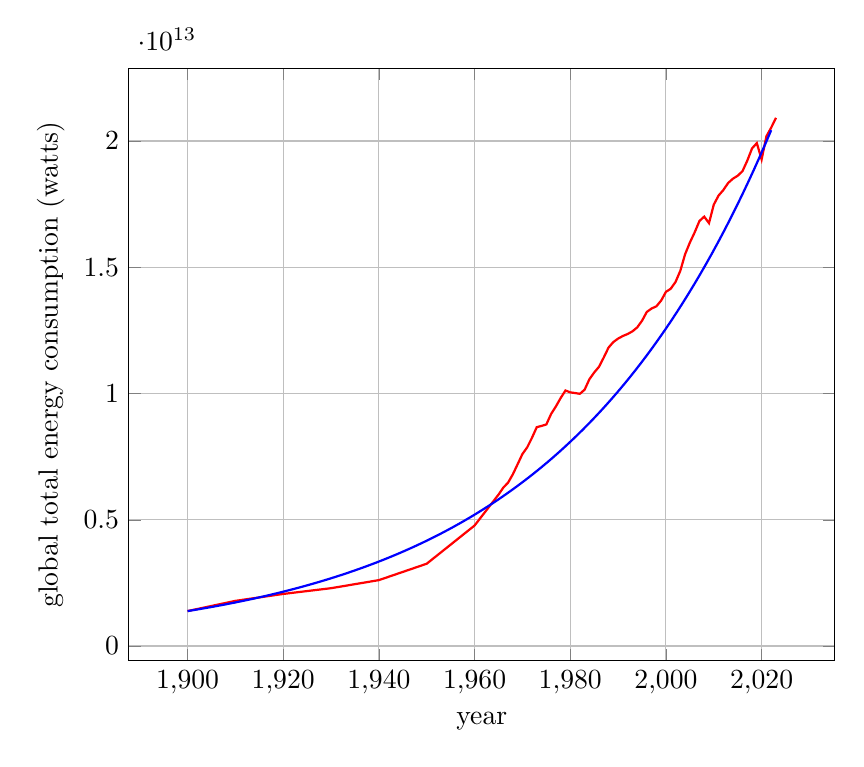
\begin{tikzpicture}
		\begin{axis}[
			width=0.87\linewidth,
			xlabel=year,
			ylabel=global total energy consumption (watts),
			%ymode=log,
			%xmin=1, xmax=100,
			%ymin=0, ymax=10,
			grid=both,
			minor grid style={gray!25},
			major grid style={gray!50},
			]
			\addplot[red, thick] coordinates {
				(1900,1384842719178.08)
				(1910,1789459664840.18)
				(1920,2063559106164.38)
				(1930,2291083207762.56)
				(1940,2610654486301.37)
				(1950,3260730593607.31)
				(1960,4773274988584.48)
				(1965,5995818389383.56)
				(1966,6272994454337.9)
				(1967,6470943432191.78)
				(1968,6801203025114.16)
				(1969,7201847321575.34)
				(1970,7603835611187.22)
				(1971,7869590803881.28)
				(1972,8248056323059.36)
				(1973,8668675863812.79)
				(1974,8716183233561.64)
				(1975,8775243811872.15)
				(1976,9191466911986.3)
				(1977,9489904755593.61)
				(1978,9824091708330.02)
				(1979,10119395099993.5)
				(1980,10046032664193.3)
				(1981,10019010932800.6)
				(1982,9987578635635.05)
				(1983,10150964744911.1)
				(1984,10566237189104.8)
				(1985,10830538633053.7)
				(1986,11057217350585.6)
				(1987,11425945962330.3)
				(1988,11818782019799.4)
				(1989,12036838443189.5)
				(1990,12175315152111.9)
				(1991,12277611525958.9)
				(1992,12357528647716.9)
				(1993,12461785556438.4)
				(1994,12619232065787.7)
				(1995,12881553615239.7)
				(1996,13230106392865.3)
				(1997,13366356573196.3)
				(1998,13452143532831.1)
				(1999,13680664873812.8)
				(2000,14026033540228.3)
				(2001,14149037323230.6)
				(2002,14415466325148.4)
				(2003,14856074400833.3)
				(2004,15512438775456.6)
				(2005,15976127636872.1)
				(2006,16379188998744.3)
				(2007,16830318881278.5)
				(2008,17004534713926.9)
				(2009,16746514823059.4)
				(2010,17479970410274)
				(2011,17838005931506.8)
				(2012,18057739672374.4)
				(2013,18336668036529.7)
				(2014,18505823052511.4)
				(2015,18624028578767.1)
				(2016,18803508173516)
				(2017,19219526810502.3)
				(2018,19706556689497.7)
				(2019,19915249691780.8)
				(2020,19266977614155.3)
				(2021,20187217933790)
				(2022,20527305490867.6)
				(2023,20916674668949.8)
			};
			\addplot[blue, thick, domain=1900:2022, samples=100]  {1384842719178.08*pow(1.022318254,x-1900)};
		\end{axis}
	\end{tikzpicture}
	
	\pagebreak
	
	Let's again stretch this out to the year 3000:
	
	\bigskip
	
	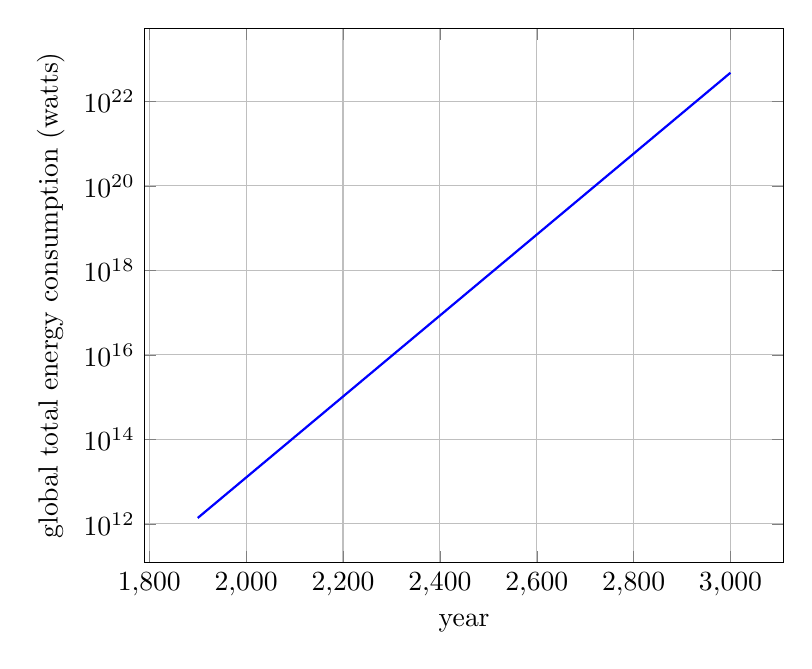
\begin{tikzpicture}
		\begin{axis}[
			width=0.8\linewidth,
			xlabel=year,
			ylabel=global total energy consumption (watts),
			ymode=log,
			%xmin=1, xmax=100,
			%ymin=0, ymax=10,
			grid=both,
			minor grid style={gray!25},
			major grid style={gray!50},
			]
			\addplot[blue, thick, domain=1900:3000, samples=100]  {1384842719178.08*pow(1.022318254,x-1900)};
		\end{axis}
	\end{tikzpicture}
	
	Here are some exact numbers that can be extracted from this:
	
	\begin{center}
		\begin{tabular}{c | c | c | c}
			year & exact & rough & kardashev level \\\hline
			2000 & 12 589 601 767 577 W & 1.26E+13 W & 0.71 \\\hline
			2050 & 37 959 262 246 954 W & 3.80E+13 W & 0.76 \\\hline
			2100 & 114 452 038 828 097 W & 1.14E+14 W & 0.81 \\\hline
			2150 & 345 087 560 097 656 W & 3.45E+14 W & 0.85 \\\hline
			2200 & 1 040 483 204 611 280 W & 1.04E+15 W & 0.90 \\\hline
			2250 & 3 137 190 163 481 378 W & 3.14E+15 W & 0.95 \\\hline
			2300 & 9 459 030 264 233 090 W & 9.46E+15 W & 1.00 \\\hline
			2350 & 28 520 188 090 985 200 W & 2.85E+16 W & 1.05 \\\hline
			2400 & 85 992 020 960 208 200 W & 8.60E+16 W & 1.09 \\\hline
			2450 & 259 276 960 068 794 000 W & 2.59E+17 W & 1.14 \\\hline
			2500 & 781 753 251 893 250 000 W & 7.82E+17 W & 1.19 \\\hline
			2600 & 7 106 916 897 888 330 000 W & 7.11E+18 W & 1.29 \\\hline
			2700 & 64 608 964 108 776 900 000 W & 6.46E+19 W & 1.38 \\\hline
			2800 & 587 359 934 439 298 000 000 W & 5.87E+20 W & 1.48 \\\hline
			2900 & 5 339 687 725 122 810 000 000 W & 5.34E+21 W & 1.57 \\\hline
			3000 & 48 543 088 028 374 600 000 000 W & 4.85E+22 W & 1.67
		\end{tabular}
	\end{center}
	
	\pagebreak
	
	\small
	
	\noindent
	\begin{tabular}{|c|c|}
		\hline
		year & Watts \\
		\hline
		2025 & 2.1861E+13 \\
		\hline
		2030 & 2.4412E+13 \\
		\hline
		2035 & 2.7260E+13 \\
		\hline
		2040 & 3.0441E+13 \\
		\hline
		2045 & 3.3993E+13 \\
		\hline
		2050 & 3.7959E+13 \\
		\hline
		2055 & 4.2389E+13 \\
		\hline
		2060 & 4.7335E+13 \\
		\hline
		2065 & 5.2858E+13 \\
		\hline
		2070 & 5.9026E+13 \\
		\hline
		2075 & 6.5913E+13 \\
		\hline
		2080 & 7.3604E+13 \\
		\hline
		2085 & 8.2192E+13 \\
		\hline
		2090 & 9.1783E+13 \\
		\hline
		2095 & 1.0249E+14 \\
		\hline
		2100 & 1.1445E+14 \\
		\hline
		2105 & 1.2781E+14 \\
		\hline
		2110 & 1.4272E+14 \\
		\hline
		2115 & 1.5937E+14 \\
		\hline
		2120 & 1.7797E+14 \\
		\hline
		2125 & 1.9874E+14 \\
		\hline
		2130 & 2.2193E+14 \\
		\hline
		2135 & 2.4782E+14 \\
		\hline
		2140 & 2.7674E+14 \\
		\hline
		2145 & 3.0903E+14 \\
		\hline
		2150 & 3.4509E+14 \\
		\hline
		2155 & 3.8535E+14 \\
		\hline
		2160 & 4.3032E+14 \\
		\hline
		2165 & 4.8053E+14 \\
		\hline
		2170 & 5.3660E+14 \\
		\hline
		2175 & 5.9921E+14 \\
		\hline
		2180 & 6.6913E+14 \\
		\hline
		2185 & 7.4721E+14 \\
		\hline
		2190 & 8.3440E+14 \\
		\hline
		2195 & 9.3176E+14 \\
		\hline
		2200 & 1.0405E+15 \\
		\hline
		2205 & 1.1619E+15 \\
		\hline
		2210 & 1.2975E+15 \\
		\hline
		2215 & 1.4489E+15 \\
		\hline
		2220 & 1.6179E+15 \\
		\hline
		2225 & 1.8067E+15 \\
		\hline
		2230 & 2.0175E+15 \\
		\hline
		2235 & 2.2529E+15 \\
		\hline
		2240 & 2.5158E+15 \\
		\hline
		2245 & 2.8094E+15 \\
		\hline
		2250 & 3.1372E+15 \\
		\hline
		2255 & 3.5033E+15 \\
		\hline
		2260 & 3.9120E+15 \\
		\hline
		2265 & 4.3685E+15 \\
		\hline
	\end{tabular}
	\hfill
	\begin{tabular}{|c|c|}
		\hline
		year & Watts \\
		\hline
		2270 & 4.8782E+15 \\
		\hline
		2275 & 5.4475E+15 \\
		\hline
		2280 & 6.0831E+15 \\
		\hline
		2285 & 6.7929E+15 \\
		\hline
		2290 & 7.5855E+15 \\
		\hline
		2295 & 8.4706E+15 \\
		\hline
		2300 & 9.4590E+15 \\
		\hline
		2305 & 1.0563E+16 \\
		\hline
		2310 & 1.1795E+16 \\
		\hline
		2315 & 1.3172E+16 \\
		\hline
		2320 & 1.4709E+16 \\
		\hline
		2325 & 1.6425E+16 \\
		\hline
		2330 & 1.8341E+16 \\
		\hline
		2335 & 2.0481E+16 \\
		\hline
		2340 & 2.2871E+16 \\
		\hline
		2345 & 2.5540E+16 \\
		\hline
		2350 & 2.8520E+16 \\
		\hline
		2355 & 3.1848E+16 \\
		\hline
		2360 & 3.5564E+16 \\
		\hline
		2365 & 3.9714E+16 \\
		\hline
		2370 & 4.4348E+16 \\
		\hline
		2375 & 4.9523E+16 \\
		\hline
		2380 & 5.5301E+16 \\
		\hline
		2385 & 6.1754E+16 \\
		\hline
		2390 & 6.8960E+16 \\
		\hline
		2395 & 7.7007E+16 \\
		\hline
		2400 & 8.5992E+16 \\
		\hline
		2405 & 9.6026E+16 \\
		\hline
		2410 & 1.0723E+17 \\
		\hline
		2415 & 1.1974E+17 \\
		\hline
		2420 & 1.3372E+17 \\
		\hline
		2425 & 1.4932E+17 \\
		\hline
		2430 & 1.6674E+17 \\
		\hline
		2435 & 1.8620E+17 \\
		\hline
		2440 & 2.0792E+17 \\
		\hline
		2445 & 2.3218E+17 \\
		\hline
		2450 & 2.5928E+17 \\
		\hline
		2455 & 2.8953E+17 \\
		\hline
		2460 & 3.2331E+17 \\
		\hline
		2465 & 3.6104E+17 \\
		\hline
		2470 & 4.0317E+17 \\
		\hline
		2475 & 4.5021E+17 \\
		\hline
		2480 & 5.0274E+17 \\
		\hline
		2485 & 5.6141E+17 \\
		\hline
		2490 & 6.2691E+17 \\
		\hline
		2495 & 7.0007E+17 \\
		\hline
		2500 & 7.8175E+17 \\
		\hline
		2505 & 8.7297E+17 \\
		\hline
		2510 & 9.7483E+17 \\
		\hline
	\end{tabular}
	\hfill
	\begin{tabular}{|c|c|}
		\hline
		year & Watts \\
		\hline
		2515 & 1.0886E+18 \\
		\hline
		2520 & 1.2156E+18 \\
		\hline
		2525 & 1.3574E+18 \\
		\hline
		2530 & 1.5158E+18 \\
		\hline
		2535 & 1.6927E+18 \\
		\hline
		2540 & 1.8902E+18 \\
		\hline
		2545 & 2.1108E+18 \\
		\hline
		2550 & 2.3571E+18 \\
		\hline
		2555 & 2.6321E+18 \\
		\hline
		2560 & 2.9393E+18 \\
		\hline
		2565 & 3.2822E+18 \\
		\hline
		2570 & 3.6652E+18 \\
		\hline
		2575 & 4.0929E+18 \\
		\hline
		2580 & 4.5704E+18 \\
		\hline
		2585 & 5.1038E+18 \\
		\hline
		2590 & 5.6993E+18 \\
		\hline
		2595 & 6.3643E+18 \\
		\hline
		2600 & 7.1069E+18 \\
		\hline
		2605 & 7.9362E+18 \\
		\hline
		2610 & 8.8622E+18 \\
		\hline
		2615 & 9.8963E+18 \\
		\hline
		2620 & 1.1051E+19 \\
		\hline
		2625 & 1.2341E+19 \\
		\hline
		2630 & 1.3780E+19 \\
		\hline
		2635 & 1.5388E+19 \\
		\hline
		2640 & 1.7184E+19 \\
		\hline
		2645 & 1.9189E+19 \\
		\hline
		2650 & 2.1428E+19 \\
		\hline
		2655 & 2.3929E+19 \\
		\hline
		2660 & 2.6721E+19 \\
		\hline
		2665 & 2.9839E+19 \\
		\hline
		2670 & 3.3320E+19 \\
		\hline
		2675 & 3.7208E+19 \\
		\hline
		2680 & 4.1550E+19 \\
		\hline
		2685 & 4.6398E+19 \\
		\hline
		2690 & 5.1812E+19 \\
		\hline
		2695 & 5.7858E+19 \\
		\hline
		2700 & 6.4609E+19 \\
		\hline
		2705 & 7.2148E+19 \\
		\hline
		2710 & 8.0566E+19 \\
		\hline
		2715 & 8.9967E+19 \\
		\hline
		2720 & 1.0047E+20 \\
		\hline
		2725 & 1.1219E+20 \\
		\hline
		2730 & 1.2528E+20 \\
		\hline
		2735 & 1.3990E+20 \\
		\hline
		2740 & 1.5622E+20 \\
		\hline
		2745 & 1.7445E+20 \\
		\hline
		2750 & 1.9480E+20 \\
		\hline
		2755 & 2.1753E+20 \\
		\hline
	\end{tabular}
	\hfill
	\begin{tabular}{|c|c|}
		\hline
		year & Watts \\
		\hline
		2760 & 2.4292E+20 \\
		\hline
		2765 & 2.7126E+20 \\
		\hline
		2770 & 3.0292E+20 \\
		\hline
		2775 & 3.3826E+20 \\
		\hline
		2780 & 3.7773E+20 \\
		\hline
		2785 & 4.2181E+20 \\
		\hline
		2790 & 4.7102E+20 \\
		\hline
		2795 & 5.2599E+20 \\
		\hline
		2800 & 5.8736E+20 \\
		\hline
		2805 & 6.5590E+20 \\
		\hline
		2810 & 7.3243E+20 \\
		\hline
		2815 & 8.1789E+20 \\
		\hline
		2820 & 9.1333E+20 \\
		\hline
		2825 & 1.0199E+21 \\
		\hline
		2830 & 1.1389E+21 \\
		\hline
		2835 & 1.2718E+21 \\
		\hline
		2840 & 1.4202E+21 \\
		\hline
		2845 & 1.5859E+21 \\
		\hline
		2850 & 1.7710E+21 \\
		\hline
		2855 & 1.9776E+21 \\
		\hline
		2860 & 2.2084E+21 \\
		\hline
		2865 & 2.4660E+21 \\
		\hline
		2870 & 2.7538E+21 \\
		\hline
		2875 & 3.0751E+21 \\
		\hline
		2880 & 3.4339E+21 \\
		\hline
		2885 & 3.8346E+21 \\
		\hline
		2890 & 4.2821E+21 \\
		\hline
		2895 & 4.7817E+21 \\
		\hline
		2900 & 5.3397E+21 \\
		\hline
		2905 & 5.9627E+21 \\
		\hline
		2910 & 6.6585E+21 \\
		\hline
		2915 & 7.4355E+21 \\
		\hline
		2920 & 8.3031E+21 \\
		\hline
		2925 & 9.2719E+21 \\
		\hline
		2930 & 1.0354E+22 \\
		\hline
		2935 & 1.1562E+22 \\
		\hline
		2940 & 1.2911E+22 \\
		\hline
		2945 & 1.4418E+22 \\
		\hline
		2950 & 1.6100E+22 \\
		\hline
		2955 & 1.7978E+22 \\
		\hline
		2960 & 2.0076E+22 \\
		\hline
		2965 & 2.2419E+22 \\
		\hline
		2970 & 2.5035E+22 \\
		\hline
		2975 & 2.7956E+22 \\
		\hline
		2980 & 3.1218E+22 \\
		\hline
		2985 & 3.4861E+22 \\
		\hline
		2990 & 3.8928E+22 \\
		\hline
		2995 & 4.3471E+22 \\
		\hline
		3000 & 4.8543E+22 \\
		\hline
	\end{tabular}
	
	\normalsize
	
	\pagebreak
	
	\small
	
	\noindent
	\begin{tabular}{|c|c|}
		\hline
		year & Kardashev \\
		\hline
		2025 & 0.734 \\
		\hline
		2030 & 0.739 \\
		\hline
		2035 & 0.744 \\
		\hline
		2040 & 0.748 \\
		\hline
		2045 & 0.753 \\
		\hline
		2050 & 0.758 \\
		\hline
		2055 & 0.763 \\
		\hline
		2060 & 0.768 \\
		\hline
		2065 & 0.772 \\
		\hline
		2070 & 0.777 \\
		\hline
		2075 & 0.782 \\
		\hline
		2080 & 0.787 \\
		\hline
		2085 & 0.791 \\
		\hline
		2090 & 0.796 \\
		\hline
		2095 & 0.801 \\
		\hline
		2100 & 0.806 \\
		\hline
		2105 & 0.811 \\
		\hline
		2110 & 0.815 \\
		\hline
		2115 & 0.820 \\
		\hline
		2120 & 0.825 \\
		\hline
		2125 & 0.830 \\
		\hline
		2130 & 0.835 \\
		\hline
		2135 & 0.839 \\
		\hline
		2140 & 0.844 \\
		\hline
		2145 & 0.849 \\
		\hline
		2150 & 0.854 \\
		\hline
		2155 & 0.859 \\
		\hline
		2160 & 0.863 \\
		\hline
		2165 & 0.868 \\
		\hline
		2170 & 0.873 \\
		\hline
		2175 & 0.878 \\
		\hline
		2180 & 0.883 \\
		\hline
		2185 & 0.887 \\
		\hline
		2190 & 0.892 \\
		\hline
		2195 & 0.897 \\
		\hline
		2200 & 0.902 \\
		\hline
		2205 & 0.907 \\
		\hline
		2210 & 0.911 \\
		\hline
		2215 & 0.916 \\
		\hline
		2220 & 0.921 \\
		\hline
		2225 & 0.926 \\
		\hline
		2230 & 0.930 \\
		\hline
		2235 & 0.935 \\
		\hline
		2240 & 0.940 \\
		\hline
		2245 & 0.945 \\
		\hline
		2250 & 0.950 \\
		\hline
		2255 & 0.954 \\
		\hline
		2260 & 0.959 \\
		\hline
		2265 & 0.964 \\
		\hline
	\end{tabular}
	\hfill
	\begin{tabular}{|c|c|}
		\hline
		year & Kardashev \\
		\hline
		2270 & 0.969 \\
		\hline
		2275 & 0.974 \\
		\hline
		2280 & 0.978 \\
		\hline
		2285 & 0.983 \\
		\hline
		2290 & 0.988 \\
		\hline
		2295 & 0.993 \\
		\hline
		2300 & 0.998 \\
		\hline
		2305 & 1.002 \\
		\hline
		2310 & 1.007 \\
		\hline
		2315 & 1.012 \\
		\hline
		2320 & 1.017 \\
		\hline
		2325 & 1.022 \\
		\hline
		2330 & 1.026 \\
		\hline
		2335 & 1.031 \\
		\hline
		2340 & 1.036 \\
		\hline
		2345 & 1.041 \\
		\hline
		2350 & 1.046 \\
		\hline
		2355 & 1.050 \\
		\hline
		2360 & 1.055 \\
		\hline
		2365 & 1.060 \\
		\hline
		2370 & 1.065 \\
		\hline
		2375 & 1.069 \\
		\hline
		2380 & 1.074 \\
		\hline
		2385 & 1.079 \\
		\hline
		2390 & 1.084 \\
		\hline
		2395 & 1.089 \\
		\hline
		2400 & 1.093 \\
		\hline
		2405 & 1.098 \\
		\hline
		2410 & 1.103 \\
		\hline
		2415 & 1.108 \\
		\hline
		2420 & 1.113 \\
		\hline
		2425 & 1.117 \\
		\hline
		2430 & 1.122 \\
		\hline
		2435 & 1.127 \\
		\hline
		2440 & 1.132 \\
		\hline
		2445 & 1.137 \\
		\hline
		2450 & 1.141 \\
		\hline
		2455 & 1.146 \\
		\hline
		2460 & 1.151 \\
		\hline
		2465 & 1.156 \\
		\hline
		2470 & 1.161 \\
		\hline
		2475 & 1.165 \\
		\hline
		2480 & 1.170 \\
		\hline
		2485 & 1.175 \\
		\hline
		2490 & 1.180 \\
		\hline
		2495 & 1.185 \\
		\hline
		2500 & 1.189 \\
		\hline
		2505 & 1.194 \\
		\hline
		2510 & 1.199 \\
		\hline
	\end{tabular}
	\hfill
	\begin{tabular}{|c|c|}
		\hline
		year & Kardashev \\
		\hline
		2515 & 1.204 \\
		\hline
		2520 & 1.208 \\
		\hline
		2525 & 1.213 \\
		\hline
		2530 & 1.218 \\
		\hline
		2535 & 1.223 \\
		\hline
		2540 & 1.228 \\
		\hline
		2545 & 1.232 \\
		\hline
		2550 & 1.237 \\
		\hline
		2555 & 1.242 \\
		\hline
		2560 & 1.247 \\
		\hline
		2565 & 1.252 \\
		\hline
		2570 & 1.256 \\
		\hline
		2575 & 1.261 \\
		\hline
		2580 & 1.266 \\
		\hline
		2585 & 1.271 \\
		\hline
		2590 & 1.276 \\
		\hline
		2595 & 1.280 \\
		\hline
		2600 & 1.285 \\
		\hline
		2605 & 1.290 \\
		\hline
		2610 & 1.295 \\
		\hline
		2615 & 1.300 \\
		\hline
		2620 & 1.304 \\
		\hline
		2625 & 1.309 \\
		\hline
		2630 & 1.314 \\
		\hline
		2635 & 1.319 \\
		\hline
		2640 & 1.324 \\
		\hline
		2645 & 1.328 \\
		\hline
		2650 & 1.333 \\
		\hline
		2655 & 1.338 \\
		\hline
		2660 & 1.343 \\
		\hline
		2665 & 1.347 \\
		\hline
		2670 & 1.352 \\
		\hline
		2675 & 1.357 \\
		\hline
		2680 & 1.362 \\
		\hline
		2685 & 1.367 \\
		\hline
		2690 & 1.371 \\
		\hline
		2695 & 1.376 \\
		\hline
		2700 & 1.381 \\
		\hline
		2705 & 1.386 \\
		\hline
		2710 & 1.391 \\
		\hline
		2715 & 1.395 \\
		\hline
		2720 & 1.400 \\
		\hline
		2725 & 1.405 \\
		\hline
		2730 & 1.410 \\
		\hline
		2735 & 1.415 \\
		\hline
		2740 & 1.419 \\
		\hline
		2745 & 1.424 \\
		\hline
		2750 & 1.429 \\
		\hline
		2755 & 1.434 \\
		\hline
	\end{tabular}
	\hfill
	\begin{tabular}{|c|c|}
		\hline
		year & Kardashev \\
		\hline
		2760 & 1.439 \\
		\hline
		2765 & 1.443 \\
		\hline
		2770 & 1.448 \\
		\hline
		2775 & 1.453 \\
		\hline
		2780 & 1.458 \\
		\hline
		2785 & 1.463 \\
		\hline
		2790 & 1.467 \\
		\hline
		2795 & 1.472 \\
		\hline
		2800 & 1.477 \\
		\hline
		2805 & 1.482 \\
		\hline
		2810 & 1.486 \\
		\hline
		2815 & 1.491 \\
		\hline
		2820 & 1.496 \\
		\hline
		2825 & 1.501 \\
		\hline
		2830 & 1.506 \\
		\hline
		2835 & 1.510 \\
		\hline
		2840 & 1.515 \\
		\hline
		2845 & 1.520 \\
		\hline
		2850 & 1.525 \\
		\hline
		2855 & 1.530 \\
		\hline
		2860 & 1.534 \\
		\hline
		2865 & 1.539 \\
		\hline
		2870 & 1.544 \\
		\hline
		2875 & 1.549 \\
		\hline
		2880 & 1.554 \\
		\hline
		2885 & 1.558 \\
		\hline
		2890 & 1.563 \\
		\hline
		2895 & 1.568 \\
		\hline
		2900 & 1.573 \\
		\hline
		2905 & 1.578 \\
		\hline
		2910 & 1.582 \\
		\hline
		2915 & 1.587 \\
		\hline
		2920 & 1.592 \\
		\hline
		2925 & 1.597 \\
		\hline
		2930 & 1.602 \\
		\hline
		2935 & 1.606 \\
		\hline
		2940 & 1.611 \\
		\hline
		2945 & 1.616 \\
		\hline
		2950 & 1.621 \\
		\hline
		2955 & 1.625 \\
		\hline
		2960 & 1.630 \\
		\hline
		2965 & 1.635 \\
		\hline
		2970 & 1.640 \\
		\hline
		2975 & 1.645 \\
		\hline
		2980 & 1.649 \\
		\hline
		2985 & 1.654 \\
		\hline
		2990 & 1.659 \\
		\hline
		2995 & 1.664 \\
		\hline
		3000 & 1.669 \\
		\hline
	\end{tabular}
	
	\normalsize
	
	\pagebreak
	
	\section{Energy consumption per person}
	
	Our World In Data does not have data on energy usage per capita from before the year 1965, so I will be extrapolating from data on total global energy use and total population, but regardless the data is still presented on the chart below in red. All converted from kilowatt-hours per year to watts.
	
	\bigskip
	
	In green, an exponential function extrapolated from population and global energy trends:
	
	
	\begin{center}
		{\large $ y = 1483.29691780822 \times 1.00904943^{x-1965} $}
	\end{center}
	
	\noindent Which represents a starting point at year 1965 with 1483.29691780822 watts per person, and growth of roughly 0.905\% per year.
	
	\medskip
	
	In blue shown is an exponential function calculated from data between years 1965 and 2023:
	
	\begin{center}
		{\large $ y = 1483.29691780822 \times 1.008634196^{x-1965} $}
	\end{center}
	
	\noindent Which represents a starting point at year 1965 with 1483.29691780822 watts per person, and growth of roughly 0.863\% per year.
	
	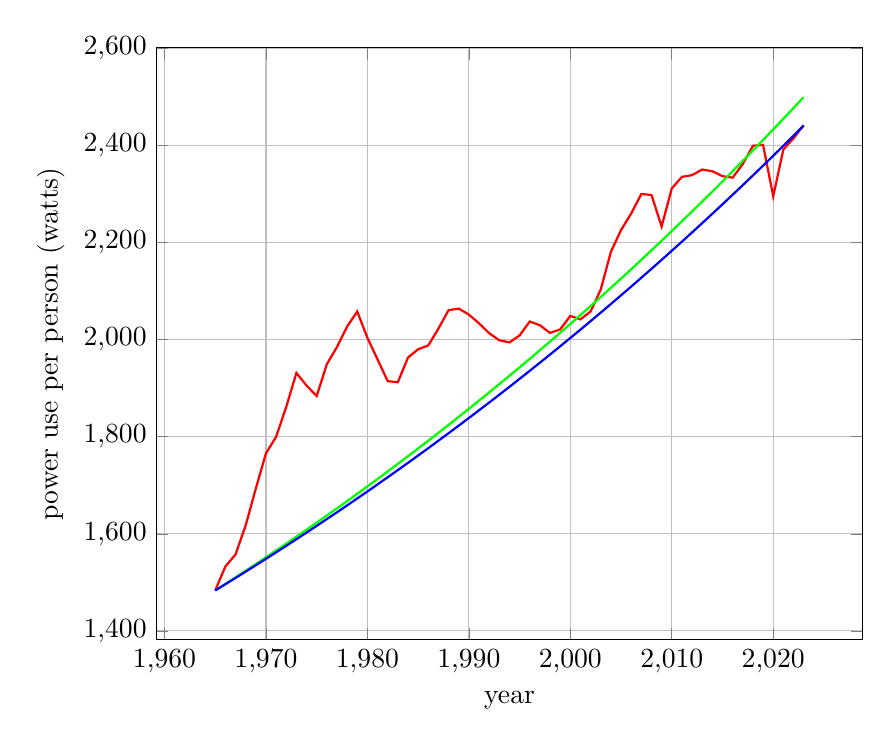
\begin{tikzpicture}
		\begin{axis}[
			width=0.87\linewidth,
			xlabel=year,
			ylabel=power use per person (watts),
			%ymode=log,
			%xmin=1, xmax=100,
			%ymin=0, ymax=10,
			grid=both,
			minor grid style={gray!25},
			major grid style={gray!50},
			]
			\addplot[red, thick] coordinates {
				(1965,1483.29691780822)
				(1966,1532.61084474886)
				(1967,1557.28630136986)
				(1968,1617.23321917808)
				(1969,1693.13869863014)
				(1970,1765.91723744292)
				(1971,1799.71780821918)
				(1972,1861.612956621)
				(1973,1931.47625570776)
				(1974,1905.41073059361)
				(1975,1883.7696347032)
				(1976,1949.47557077626)
				(1977,1984.86974885845)
				(1978,2027.09737442922)
				(1979,2057.99543378995)
				(1980,2003.7049086758)
				(1981,1959.35650684932)
				(1982,1914.4401826484)
				(1983,1912.40216894977)
				(1984,1963.13207762557)
				(1985,1980.20605022831)
				(1986,1988.0801369863)
				(1987,2022.83196347032)
				(1988,2060.84965753425)
				(1989,2063.99543378995)
				(1990,2051.65068493151)
				(1991,2033.60422374429)
				(1992,2013.38630136986)
				(1993,1998.72283105023)
				(1994,1994.38436073059)
				(1995,2008.6700913242)
				(1996,2037.51221461187)
				(1997,2029.79714611872)
				(1998,2013.99589041096)
				(1999,2021.09908675799)
				(2000,2048.9997716895)
				(2001,2041.8252283105)
				(2002,2058.16095890411)
				(2003,2103.35753424658)
				(2004,2181.10776255708)
				(2005,2225.86107305936)
				(2006,2260.07888127854)
				(2007,2300.13892694064)
				(2008,2298.16746575342)
				(2009,2233.23401826484)
				(2010,2311.62865296804)
				(2011,2335.48401826484)
				(2012,2339.06655251142)
				(2013,2350.60616438356)
				(2014,2347.04577625571)
				(2015,2336.95844748858)
				(2016,2333.824543379)
				(2017,2362.04851598174)
				(2018,2399.6203196347)
				(2019,2401.41506849315)
				(2020,2295.46050228311)
				(2021,2391.975456621)
				(2022,2414.88070776256)
				(2023,2442.20433789954)
			};
			\addplot[green, thick, domain=1965:2023, samples=100]  {1483.29691780822*pow(1.00904943,x-1965)};
			\addplot[blue, thick, domain=1965:2023, samples=100]  {1483.29691780822*pow(1.008634196,x-1965)};
		\end{axis}
	\end{tikzpicture}
	
	It's noticeable that the real data shows growth, but it is not clear of what kind, personally from eyeballing it I would say maybe even logarhythmic rather than exponential, but this document focusses on exponential growth.
	
	\medskip
	
	It is important to note though that 0.905\% growth is more consistent with the growth I presented earlier for global energy use and total population size.
	
	\pagebreak
	
	Extending the growth trend all the way to the year 3000,\newline again 0.905\% in green \& 0.863\% in blue:
	
	\medskip
	
	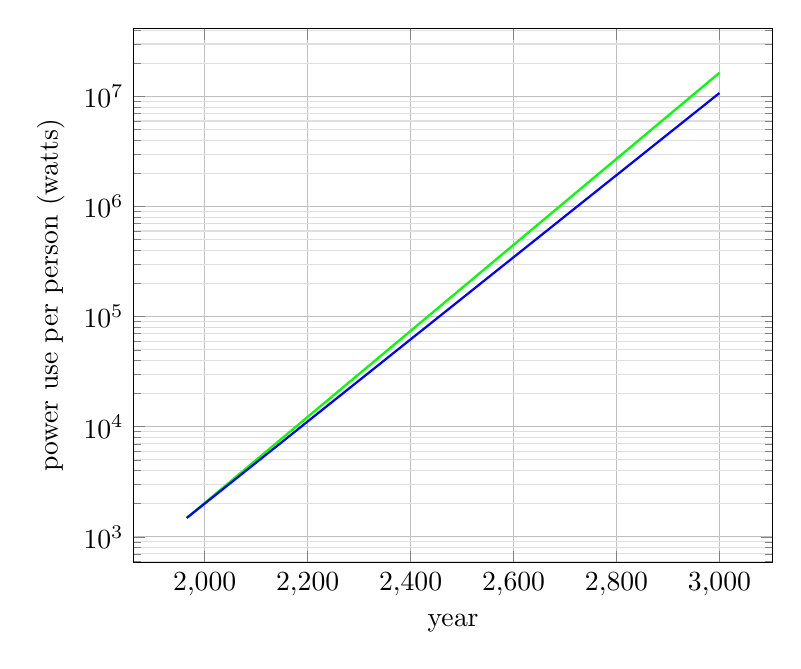
\begin{tikzpicture}
		\begin{axis}[
			width=0.8\linewidth,
			xlabel=year,
			ylabel=power use per person (watts),
			ymode=log,
			%xmin=1, xmax=100,
			%ymin=0, ymax=10,
			grid=both,
			minor grid style={gray!25},
			major grid style={gray!50},
			]
			\addplot[green, thick, domain=1965:3000, samples=100]  {1483.29691780822*pow(1.00904943,x-1965)};
			\addplot[blue, thick, domain=1965:3000, samples=100]  {1483.29691780822*pow(1.008634196,x-1965)};
		\end{axis}
	\end{tikzpicture}

	Here are some exact numbers to be extracted from this:
	
	\bigskip
	
	\noindent
	\begin{minipage}{0.5\textwidth}
		
		\begin{center}
			0.905\% annual growth
			
			\medskip
			
			\small
			\begin{tabular}{c | c | c}
				year & exact & rough\\\hline
				2000 & 2033 W & 2.03$\times 10^{3}$ W \\\hline
				2050 & 3190 W & 3.19$\times 10^{3}$ W \\\hline
				2100 & 5005 W & 5.01$\times 10^{3}$ W \\\hline
				2150 & 7853 W & 7.85$\times 10^{3}$ W \\\hline
				2200 & 12321 W & 1.23$\times 10^{4}$ W \\\hline
				2250 & 19332 W & 1.93$\times 10^{4}$ W \\\hline
				2300 & 30332 W & 3.03$\times 10^{4}$ W \\\hline
				2350 & 47590 W & 4.76$\times 10^{4}$ W \\\hline
				2400 & 74669 W & 7.47$\times 10^{4}$ W \\\hline
				2450 & 117155 W & 1.17$\times 10^{5}$ W \\\hline
				2500 & 183816 W & 1.84$\times 10^{5}$ W \\\hline
				2600 & 452510 W & 4.53$\times 10^{5}$ W \\\hline
				2700 & 1113968 W & 1.11$\times 10^{6}$ W \\\hline
				2800 & 2742311 W & 2.74$\times 10^{6}$ W \\\hline
				2900 & 6750887 W & 6.75$\times 10^{6}$ W \\\hline
				3000 & 16619003 W & 1.66$\times 10^{7}$ W
			\end{tabular}
		\end{center}
	\end{minipage}\vline\nobreak
	\begin{minipage}{0.5\textwidth}
		
		\begin{center}
			0.863\% annual growth
			
			\medskip
		
			\small
			\begin{tabular}{c | c | c}
				year & exact & rough\\\hline
				2000 & 2004 W & 2.00$\times 10^{3}$ W \\\hline
				2050 & 3080 W & 3.08$\times 10^{3}$ W \\\hline
				2100 & 4735 W & 4.73$\times 10^{3}$ W \\\hline
				2150 & 7277 W & 7.28$\times 10^{3}$ W \\\hline
				2200 & 11185 W & 1.12$\times 10^{4}$ W \\\hline
				2250 & 17192 W & 1.72$\times 10^{4}$ W \\\hline
				2300 & 26425 W & 2.64$\times 10^{4}$ W \\\hline
				2350 & 40616 W & 4.06$\times 10^{4}$ W \\\hline
				2400 & 62428 W & 6.24$\times 10^{4}$ W \\\hline
				2450 & 95955 W & 9.60$\times 10^{4}$ W \\\hline
				2500 & 147486 W & 1.47$\times 10^{5}$ W \\\hline
				2600 & 348434 W & 3.48$\times 10^{5}$ W \\\hline
				2700 & 823169 W & 8.23$\times 10^{5}$ W \\\hline
				2800 & 1944722 W & 1.94$\times 10^{6}$ W \\\hline
				2900 & 4594375 W & 4.59$\times 10^{6}$ W \\\hline
				3000 & 10854136 W & 1.09$\times 10^{7}$ W
				
			\end{tabular}
		\end{center}
	\end{minipage}
	
	\pagebreak
	
	\small
	
	\noindent
	\begin{tabular}{|c|c|}
		\hline
		year & W (0.905\%) \\
		\hline
		2025 & 4.5739E+03 \\
		\hline
		2030 & 4.7846E+03 \\
		\hline
		2035 & 5.0050E+03 \\
		\hline
		2040 & 5.2356E+03 \\
		\hline
		2045 & 5.4769E+03 \\
		\hline
		2050 & 5.7292E+03 \\
		\hline
		2055 & 5.9932E+03 \\
		\hline
		2060 & 6.2693E+03 \\
		\hline
		2065 & 6.5581E+03 \\
		\hline
		2070 & 6.8603E+03 \\
		\hline
		2075 & 7.1764E+03 \\
		\hline
		2080 & 7.5070E+03 \\
		\hline
		2085 & 7.8529E+03 \\
		\hline
		2090 & 8.2147E+03 \\
		\hline
		2095 & 8.5932E+03 \\
		\hline
		2100 & 8.9891E+03 \\
		\hline
		2105 & 9.4033E+03 \\
		\hline
		2110 & 9.8365E+03 \\
		\hline
		2115 & 1.0290E+04 \\
		\hline
		2120 & 1.0764E+04 \\
		\hline
		2125 & 1.1260E+04 \\
		\hline
		2130 & 1.1778E+04 \\
		\hline
		2135 & 1.2321E+04 \\
		\hline
		2140 & 1.2889E+04 \\
		\hline
		2145 & 1.3483E+04 \\
		\hline
		2150 & 1.4104E+04 \\
		\hline
		2155 & 1.4754E+04 \\
		\hline
		2160 & 1.5433E+04 \\
		\hline
		2165 & 1.6145E+04 \\
		\hline
		2170 & 1.6888E+04 \\
		\hline
		2175 & 1.7666E+04 \\
		\hline
		2180 & 1.8480E+04 \\
		\hline
		2185 & 1.9332E+04 \\
		\hline
		2190 & 2.0223E+04 \\
		\hline
		2195 & 2.1154E+04 \\
		\hline
		2200 & 2.2129E+04 \\
		\hline
		2205 & 2.3148E+04 \\
		\hline
		2210 & 2.4215E+04 \\
		\hline
		2215 & 2.5331E+04 \\
		\hline
		2220 & 2.6498E+04 \\
		\hline
		2225 & 2.7719E+04 \\
		\hline
		2230 & 2.8996E+04 \\
		\hline
		2235 & 3.0332E+04 \\
		\hline
		2240 & 3.1729E+04 \\
		\hline
		2245 & 3.3191E+04 \\
		\hline
		2250 & 3.4720E+04 \\
		\hline
		2255 & 3.6320E+04 \\
		\hline
		2260 & 3.7993E+04 \\
		\hline
		2265 & 3.9744E+04 \\
		\hline
	\end{tabular}
	\hfill
	\begin{tabular}{|c|c|}
		\hline
		year & W (0.905\%) \\
		\hline
		2270 & 4.1575E+04 \\
		\hline
		2275 & 4.3490E+04 \\
		\hline
		2280 & 4.5494E+04 \\
		\hline
		2285 & 4.7590E+04 \\
		\hline
		2290 & 4.9783E+04 \\
		\hline
		2295 & 5.2077E+04 \\
		\hline
		2300 & 5.4476E+04 \\
		\hline
		2305 & 5.6986E+04 \\
		\hline
		2310 & 5.9611E+04 \\
		\hline
		2315 & 6.2358E+04 \\
		\hline
		2320 & 6.5231E+04 \\
		\hline
		2325 & 6.8236E+04 \\
		\hline
		2330 & 7.1380E+04 \\
		\hline
		2335 & 7.4669E+04 \\
		\hline
		2340 & 7.8109E+04 \\
		\hline
		2345 & 8.1708E+04 \\
		\hline
		2350 & 8.5473E+04 \\
		\hline
		2355 & 8.9411E+04 \\
		\hline
		2360 & 9.3530E+04 \\
		\hline
		2365 & 9.7839E+04 \\
		\hline
		2370 & 1.0235E+05 \\
		\hline
		2375 & 1.0706E+05 \\
		\hline
		2380 & 1.1200E+05 \\
		\hline
		2385 & 1.1716E+05 \\
		\hline
		2390 & 1.2255E+05 \\
		\hline
		2395 & 1.2820E+05 \\
		\hline
		2400 & 1.3411E+05 \\
		\hline
		2405 & 1.4028E+05 \\
		\hline
		2410 & 1.4675E+05 \\
		\hline
		2415 & 1.5351E+05 \\
		\hline
		2420 & 1.6058E+05 \\
		\hline
		2425 & 1.6798E+05 \\
		\hline
		2430 & 1.7572E+05 \\
		\hline
		2435 & 1.8382E+05 \\
		\hline
		2440 & 1.9229E+05 \\
		\hline
		2445 & 2.0114E+05 \\
		\hline
		2450 & 2.1041E+05 \\
		\hline
		2455 & 2.2011E+05 \\
		\hline
		2460 & 2.3025E+05 \\
		\hline
		2465 & 2.4086E+05 \\
		\hline
		2470 & 2.5195E+05 \\
		\hline
		2475 & 2.6356E+05 \\
		\hline
		2480 & 2.7570E+05 \\
		\hline
		2485 & 2.8841E+05 \\
		\hline
		2490 & 3.0170E+05 \\
		\hline
		2495 & 3.1560E+05 \\
		\hline
		2500 & 3.3014E+05 \\
		\hline
		2505 & 3.4535E+05 \\
		\hline
		2510 & 3.6126E+05 \\
		\hline
	\end{tabular}
	\hfill
	\begin{tabular}{|c|c|}
		\hline
		year & W (0.905\%) \\
		\hline
		2515 & 3.7790E+05 \\
		\hline
		2520 & 3.9531E+05 \\
		\hline
		2525 & 4.1353E+05 \\
		\hline
		2530 & 4.3258E+05 \\
		\hline
		2535 & 4.5251E+05 \\
		\hline
		2540 & 4.7336E+05 \\
		\hline
		2545 & 4.9517E+05 \\
		\hline
		2550 & 5.1798E+05 \\
		\hline
		2555 & 5.4185E+05 \\
		\hline
		2560 & 5.6681E+05 \\
		\hline
		2565 & 5.9293E+05 \\
		\hline
		2570 & 6.2025E+05 \\
		\hline
		2575 & 6.4882E+05 \\
		\hline
		2580 & 6.7872E+05 \\
		\hline
		2585 & 7.0999E+05 \\
		\hline
		2590 & 7.4270E+05 \\
		\hline
		2595 & 7.7692E+05 \\
		\hline
		2600 & 8.1271E+05 \\
		\hline
		2605 & 8.5016E+05 \\
		\hline
		2610 & 8.8933E+05 \\
		\hline
		2615 & 9.3030E+05 \\
		\hline
		2620 & 9.7316E+05 \\
		\hline
		2625 & 1.0180E+06 \\
		\hline
		2630 & 1.0649E+06 \\
		\hline
		2635 & 1.1140E+06 \\
		\hline
		2640 & 1.1653E+06 \\
		\hline
		2645 & 1.2190E+06 \\
		\hline
		2650 & 1.2751E+06 \\
		\hline
		2655 & 1.3339E+06 \\
		\hline
		2660 & 1.3954E+06 \\
		\hline
		2665 & 1.4596E+06 \\
		\hline
		2670 & 1.5269E+06 \\
		\hline
		2675 & 1.5972E+06 \\
		\hline
		2680 & 1.6708E+06 \\
		\hline
		2685 & 1.7478E+06 \\
		\hline
		2690 & 1.8283E+06 \\
		\hline
		2695 & 1.9126E+06 \\
		\hline
		2700 & 2.0007E+06 \\
		\hline
		2705 & 2.0929E+06 \\
		\hline
		2710 & 2.1893E+06 \\
		\hline
		2715 & 2.2902E+06 \\
		\hline
		2720 & 2.3957E+06 \\
		\hline
		2725 & 2.5061E+06 \\
		\hline
		2730 & 2.6215E+06 \\
		\hline
		2735 & 2.7423E+06 \\
		\hline
		2740 & 2.8687E+06 \\
		\hline
		2745 & 3.0008E+06 \\
		\hline
		2750 & 3.1391E+06 \\
		\hline
		2755 & 3.2837E+06 \\
		\hline
	\end{tabular}
	\hfill
	\begin{tabular}{|c|c|}
		\hline
		year & W (0.905\%) \\
		\hline
		2760 & 3.4350E+06 \\
		\hline
		2765 & 3.5933E+06 \\
		\hline
		2770 & 3.7588E+06 \\
		\hline
		2775 & 3.9320E+06 \\
		\hline
		2780 & 4.1132E+06 \\
		\hline
		2785 & 4.3027E+06 \\
		\hline
		2790 & 4.5009E+06 \\
		\hline
		2795 & 4.7083E+06 \\
		\hline
		2800 & 4.9252E+06 \\
		\hline
		2805 & 5.1521E+06 \\
		\hline
		2810 & 5.3895E+06 \\
		\hline
		2815 & 5.6378E+06 \\
		\hline
		2820 & 5.8976E+06 \\
		\hline
		2825 & 6.1693E+06 \\
		\hline
		2830 & 6.4535E+06 \\
		\hline
		2835 & 6.7509E+06 \\
		\hline
		2840 & 7.0619E+06 \\
		\hline
		2845 & 7.3873E+06 \\
		\hline
		2850 & 7.7276E+06 \\
		\hline
		2855 & 8.0837E+06 \\
		\hline
		2860 & 8.4561E+06 \\
		\hline
		2865 & 8.8457E+06 \\
		\hline
		2870 & 9.2533E+06 \\
		\hline
		2875 & 9.6796E+06 \\
		\hline
		2880 & 1.0126E+07 \\
		\hline
		2885 & 1.0592E+07 \\
		\hline
		2890 & 1.1080E+07 \\
		\hline
		2895 & 1.1591E+07 \\
		\hline
		2900 & 1.2125E+07 \\
		\hline
		2905 & 1.2683E+07 \\
		\hline
		2910 & 1.3268E+07 \\
		\hline
		2915 & 1.3879E+07 \\
		\hline
		2920 & 1.4518E+07 \\
		\hline
		2925 & 1.5187E+07 \\
		\hline
		2930 & 1.5887E+07 \\
		\hline
		2935 & 1.6619E+07 \\
		\hline
		2940 & 1.7385E+07 \\
		\hline
		2945 & 1.8186E+07 \\
		\hline
		2950 & 1.9024E+07 \\
		\hline
		2955 & 1.9900E+07 \\
		\hline
		2960 & 2.0817E+07 \\
		\hline
		2965 & 2.1776E+07 \\
		\hline
		2970 & 2.2779E+07 \\
		\hline
		2975 & 2.3829E+07 \\
		\hline
		2980 & 2.4927E+07 \\
		\hline
		2985 & 2.6075E+07 \\
		\hline
		2990 & 2.7277E+07 \\
		\hline
		2995 & 2.8533E+07 \\
		\hline
		3000 & 2.9848E+07 \\
		\hline
	\end{tabular}
	
	\normalsize
	
	\pagebreak
	
	\small
	
	\noindent
	\begin{tabular}{|c|c|}
		\hline
		year & W (0.863\%) \\
		\hline
		2025 & 4.3445E+03 \\
		\hline
		2030 & 4.5353E+03 \\
		\hline
		2035 & 4.7345E+03 \\
		\hline
		2040 & 4.9425E+03 \\
		\hline
		2045 & 5.1596E+03 \\
		\hline
		2050 & 5.3862E+03 \\
		\hline
		2055 & 5.6228E+03 \\
		\hline
		2060 & 5.8697E+03 \\
		\hline
		2065 & 6.1275E+03 \\
		\hline
		2070 & 6.3967E+03 \\
		\hline
		2075 & 6.6776E+03 \\
		\hline
		2080 & 6.9709E+03 \\
		\hline
		2085 & 7.2771E+03 \\
		\hline
		2090 & 7.5968E+03 \\
		\hline
		2095 & 7.9304E+03 \\
		\hline
		2100 & 8.2788E+03 \\
		\hline
		2105 & 8.6424E+03 \\
		\hline
		2110 & 9.0220E+03 \\
		\hline
		2115 & 9.4183E+03 \\
		\hline
		2120 & 9.8319E+03 \\
		\hline
		2125 & 1.0264E+04 \\
		\hline
		2130 & 1.0715E+04 \\
		\hline
		2135 & 1.1185E+04 \\
		\hline
		2140 & 1.1677E+04 \\
		\hline
		2145 & 1.2189E+04 \\
		\hline
		2150 & 1.2725E+04 \\
		\hline
		2155 & 1.3284E+04 \\
		\hline
		2160 & 1.3867E+04 \\
		\hline
		2165 & 1.4476E+04 \\
		\hline
		2170 & 1.5112E+04 \\
		\hline
		2175 & 1.5776E+04 \\
		\hline
		2180 & 1.6469E+04 \\
		\hline
		2185 & 1.7192E+04 \\
		\hline
		2190 & 1.7947E+04 \\
		\hline
		2195 & 1.8736E+04 \\
		\hline
		2200 & 1.9558E+04 \\
		\hline
		2205 & 2.0418E+04 \\
		\hline
		2210 & 2.1314E+04 \\
		\hline
		2215 & 2.2251E+04 \\
		\hline
		2220 & 2.3228E+04 \\
		\hline
		2225 & 2.4248E+04 \\
		\hline
		2230 & 2.5313E+04 \\
		\hline
		2235 & 2.6425E+04 \\
		\hline
		2240 & 2.7586E+04 \\
		\hline
		2245 & 2.8797E+04 \\
		\hline
		2250 & 3.0062E+04 \\
		\hline
		2255 & 3.1382E+04 \\
		\hline
		2260 & 3.2761E+04 \\
		\hline
		2265 & 3.4200E+04 \\
		\hline
	\end{tabular}
	\hfill
	\begin{tabular}{|c|c|}
		\hline
		year & W (0.863\%) \\
		\hline
		2270 & 3.5702E+04 \\
		\hline
		2275 & 3.7270E+04 \\
		\hline
		2280 & 3.8907E+04 \\
		\hline
		2285 & 4.0616E+04 \\
		\hline
		2290 & 4.2400E+04 \\
		\hline
		2295 & 4.4262E+04 \\
		\hline
		2300 & 4.6207E+04 \\
		\hline
		2305 & 4.8236E+04 \\
		\hline
		2310 & 5.0355E+04 \\
		\hline
		2315 & 5.2566E+04 \\
		\hline
		2320 & 5.4875E+04 \\
		\hline
		2325 & 5.7286E+04 \\
		\hline
		2330 & 5.9802E+04 \\
		\hline
		2335 & 6.2428E+04 \\
		\hline
		2340 & 6.5170E+04 \\
		\hline
		2345 & 6.8033E+04 \\
		\hline
		2350 & 7.1021E+04 \\
		\hline
		2355 & 7.4141E+04 \\
		\hline
		2360 & 7.7397E+04 \\
		\hline
		2365 & 8.0797E+04 \\
		\hline
		2370 & 8.4345E+04 \\
		\hline
		2375 & 8.8050E+04 \\
		\hline
		2380 & 9.1918E+04 \\
		\hline
		2385 & 9.5955E+04 \\
		\hline
		2390 & 1.0017E+05 \\
		\hline
		2395 & 1.0457E+05 \\
		\hline
		2400 & 1.0916E+05 \\
		\hline
		2405 & 1.1396E+05 \\
		\hline
		2410 & 1.1896E+05 \\
		\hline
		2415 & 1.2419E+05 \\
		\hline
		2420 & 1.2964E+05 \\
		\hline
		2425 & 1.3534E+05 \\
		\hline
		2430 & 1.4128E+05 \\
		\hline
		2435 & 1.4749E+05 \\
		\hline
		2440 & 1.5396E+05 \\
		\hline
		2445 & 1.6073E+05 \\
		\hline
		2450 & 1.6779E+05 \\
		\hline
		2455 & 1.7516E+05 \\
		\hline
		2460 & 1.8285E+05 \\
		\hline
		2465 & 1.9088E+05 \\
		\hline
		2470 & 1.9926E+05 \\
		\hline
		2475 & 2.0802E+05 \\
		\hline
		2480 & 2.1715E+05 \\
		\hline
		2485 & 2.2669E+05 \\
		\hline
		2490 & 2.3665E+05 \\
		\hline
		2495 & 2.4704E+05 \\
		\hline
		2500 & 2.5789E+05 \\
		\hline
		2505 & 2.6922E+05 \\
		\hline
		2510 & 2.8105E+05 \\
		\hline
	\end{tabular}
	\hfill
	\begin{tabular}{|c|c|}
		\hline
		year & W (0.863\%) \\
		\hline
		2515 & 2.9339E+05 \\
		\hline
		2520 & 3.0628E+05 \\
		\hline
		2525 & 3.1973E+05 \\
		\hline
		2530 & 3.3377E+05 \\
		\hline
		2535 & 3.4843E+05 \\
		\hline
		2540 & 3.6374E+05 \\
		\hline
		2545 & 3.7971E+05 \\
		\hline
		2550 & 3.9639E+05 \\
		\hline
		2555 & 4.1380E+05 \\
		\hline
		2560 & 4.3198E+05 \\
		\hline
		2565 & 4.5095E+05 \\
		\hline
		2570 & 4.7076E+05 \\
		\hline
		2575 & 4.9144E+05 \\
		\hline
		2580 & 5.1302E+05 \\
		\hline
		2585 & 5.3556E+05 \\
		\hline
		2590 & 5.5908E+05 \\
		\hline
		2595 & 5.8363E+05 \\
		\hline
		2600 & 6.0927E+05 \\
		\hline
		2605 & 6.3603E+05 \\
		\hline
		2610 & 6.6397E+05 \\
		\hline
		2615 & 6.9313E+05 \\
		\hline
		2620 & 7.2357E+05 \\
		\hline
		2625 & 7.5536E+05 \\
		\hline
		2630 & 7.8853E+05 \\
		\hline
		2635 & 8.2317E+05 \\
		\hline
		2640 & 8.5932E+05 \\
		\hline
		2645 & 8.9707E+05 \\
		\hline
		2650 & 9.3647E+05 \\
		\hline
		2655 & 9.7760E+05 \\
		\hline
		2660 & 1.0205E+06 \\
		\hline
		2665 & 1.0654E+06 \\
		\hline
		2670 & 1.1122E+06 \\
		\hline
		2675 & 1.1610E+06 \\
		\hline
		2680 & 1.2120E+06 \\
		\hline
		2685 & 1.2652E+06 \\
		\hline
		2690 & 1.3208E+06 \\
		\hline
		2695 & 1.3788E+06 \\
		\hline
		2700 & 1.4394E+06 \\
		\hline
		2705 & 1.5026E+06 \\
		\hline
		2710 & 1.5686E+06 \\
		\hline
		2715 & 1.6375E+06 \\
		\hline
		2720 & 1.7094E+06 \\
		\hline
		2725 & 1.7845E+06 \\
		\hline
		2730 & 1.8629E+06 \\
		\hline
		2735 & 1.9447E+06 \\
		\hline
		2740 & 2.0301E+06 \\
		\hline
		2745 & 2.1193E+06 \\
		\hline
		2750 & 2.2124E+06 \\
		\hline
		2755 & 2.3096E+06 \\
		\hline
	\end{tabular}
	\hfill
	\begin{tabular}{|c|c|}
		\hline
		year & W (0.863\%) \\
		\hline
		2760 & 2.4110E+06 \\
		\hline
		2765 & 2.5169E+06 \\
		\hline
		2770 & 2.6275E+06 \\
		\hline
		2775 & 2.7429E+06 \\
		\hline
		2780 & 2.8633E+06 \\
		\hline
		2785 & 2.9891E+06 \\
		\hline
		2790 & 3.1204E+06 \\
		\hline
		2795 & 3.2575E+06 \\
		\hline
		2800 & 3.4005E+06 \\
		\hline
		2805 & 3.5499E+06 \\
		\hline
		2810 & 3.7058E+06 \\
		\hline
		2815 & 3.8686E+06 \\
		\hline
		2820 & 4.0385E+06 \\
		\hline
		2825 & 4.2159E+06 \\
		\hline
		2830 & 4.4011E+06 \\
		\hline
		2835 & 4.5944E+06 \\
		\hline
		2840 & 4.7962E+06 \\
		\hline
		2845 & 5.0068E+06 \\
		\hline
		2850 & 5.2268E+06 \\
		\hline
		2855 & 5.4563E+06 \\
		\hline
		2860 & 5.6960E+06 \\
		\hline
		2865 & 5.9462E+06 \\
		\hline
		2870 & 6.2073E+06 \\
		\hline
		2875 & 6.4800E+06 \\
		\hline
		2880 & 6.7646E+06 \\
		\hline
		2885 & 7.0617E+06 \\
		\hline
		2890 & 7.3719E+06 \\
		\hline
		2895 & 7.6957E+06 \\
		\hline
		2900 & 8.0337E+06 \\
		\hline
		2905 & 8.3866E+06 \\
		\hline
		2910 & 8.7549E+06 \\
		\hline
		2915 & 9.1395E+06 \\
		\hline
		2920 & 9.5409E+06 \\
		\hline
		2925 & 9.9600E+06 \\
		\hline
		2930 & 1.0397E+07 \\
		\hline
		2935 & 1.0854E+07 \\
		\hline
		2940 & 1.1331E+07 \\
		\hline
		2945 & 1.1829E+07 \\
		\hline
		2950 & 1.2348E+07 \\
		\hline
		2955 & 1.2890E+07 \\
		\hline
		2960 & 1.3457E+07 \\
		\hline
		2965 & 1.4048E+07 \\
		\hline
		2970 & 1.4665E+07 \\
		\hline
		2975 & 1.5309E+07 \\
		\hline
		2980 & 1.5981E+07 \\
		\hline
		2985 & 1.6683E+07 \\
		\hline
		2990 & 1.7416E+07 \\
		\hline
		2995 & 1.8181E+07 \\
		\hline
		3000 & 1.8980E+07 \\
		\hline
	\end{tabular}
	
	\normalsize
	
	\pagebreak
	
\end{document}